%  LaTeX support: latex@mdpi.com 
%  For support, please attach all files needed for compiling as well as the log file, and specify your operating system, LaTeX version, and LaTeX editor.

%=================================================================
\documentclass[mathematics,article,submit,pdftex,moreauthors]{Definitions/mdpi} 

% Required for Algorithm 1 (the injection pseudocode); not loaded by the class.
\usepackage{algorithm}
\usepackage{algpseudocode}
%\documentclass[preprints,article,submit,moreauthors]{Definitions/mdpi} 
% For posting an early version of this manuscript as a preprint, you may use "preprints" as the journal. Changing "submit" to "accept" before posting will remove line numbers.

%--------------------
% Class Options:
%--------------------
%----------
% journal
%----------
% Choose between the following MDPI journals:
% accountaudit, acn, acoustics, actuators, addictions, addictprev, adhesives, adolescents, aerobiology, aerospace, agriculture, agriengineering, agrochemicals, agronomy, ai, aichem, aieng, aimater, aimed, aipa, air, aisens, aisoc, algorithms, allergies, alloys, amh, analog, analytica, analytics, anatomia, anesthres, animals, antibiotics, antibodies, antioxidants, applbiosci, appliedchem, appliedmath, appliedphys, applmech, applmicrobiol, applnano, applsci, aps, aquacj, archaeolstud, architecture, arm, arthropoda, asc, asi, astronautics, astronomy, atmosphere, atoms, audiolres, automation, axioms, bacteria, batteries, bdcc, beverages, biochem, bioengineering, biologics, biology, biomass, biomechanics, biomed, biomedicines, biomedinformatics, biomimetics, biomolecules, biophysica, bioresourbioprod, biosensors, biosphere, biotech, birds, blockchains, bloods, blsf, brainsci, breath, buildings, cancers, carbon, cardio, cardiogenetics, cardiovascmed, catalysts, cells, ceramics, challenges, chemengineering, chemistry, chemosensors, chemproc, children, chips, cimb, civileng, cleantechnol, climate, clinbioenerg, clinpract, clockssleep, cmd, cmtr, coasts, coatings, colloids, colorants, commodities, complexities, complications, compounds, computation, computers, condensedmatter, conservation, constrmater, cosmetics, covid, crops, cryo, cryptography, crystals, csmf, ctn, culture, curroncol, cyber, dairy, data, ddc, dentistry, dermato, dermatopathology, designs, devices, dhi, diabetology, diagnostics, dietetics, digital, disabilities, diseases, diversity, dna, drones, drugreact, drylands, dynamics, earth, ebj, ecm, ecologies, edm, eesp, electricity, electrochem, electronicmat, electronics, embodiedintell, encyclopedia, endocrines, energies, eng, engproc, entomology, entropy, environments, environremediat, epidemiologia, epigenomes, esa, est, fermentation, fibers, fintech, fire, fishes, fluids, foodeng, foods, forecasting, forensicsci, forests, fossstud, foundations, fractalfract, freshwater, fuels, future, futureinternet, futurepharmacol, futurephys, futuretransp, galaxies, gases, gastroent, gastrointestdisord, gastronomy, gels, genes, geochem, geographies, geohazards, geomatics, geometry, geosciences, geotechnics, geriatrics, germs, glacies, grainsci, grasses, green, greenhealth, gucdd, gynecolcancer, hardware, hazardousmatters, healthcare, healthcmater, hearts, hemato, hematolrep, hep, heritage, higheredu, highthroughput, horticulturae, hospitals, hydrobiology, hydrogen, hydrology, hydrometeorology, hydropower, hygiene, idr, iic, ijem, ijerph, ijgi, ijmd, ijms, ijns, ijom, ijp, ijpb, ijt, ijtm, ijtpp, ijtst, ime, immuno, industries, inflammj, informatics, information, infrastructures, inorganics, insects, instruments, inventions, iot, j, jaestheticmed, jal, japma, jcdd, jcm, jcp, jcrm, jcs, jcto, jdad, jdb, jdream, jemr, jeta, jfb, jfmk, jfth, jgbg, jgg, jimaging, jlpea, jmahp, jmmp, jmms, jmp, jmse, jne, jnt, jof, joi, joitmc, joma, jop, joptm, jor, jox, jpbi, jphytomed, jpm, jsan, jtaer, jvd, jzbg, kidneydial, kinasesphosphatases, knowledge, labmed, laboratories, lam, land, lasers, legumes, life, lights, limnolrev, lipidology, liquids, livers, logics, logistics, lubricants, lymphatics, machines, macromol, magnetism, magnetochemistry, make, marinedrugs, maritime, materials, materproc, mathematics, mca, mcb, measurements, medicina, medicines, medsci, membranes, merits, metabolites, metals, meteorology, methane, metrics, metrology, micro, microarrays, microbiolres, microelectronics, micromachines, microorganisms, microplastics, microwave, minerals, mining, mmphys, modelling, molbank, molecules, mollusca, mps, msf, mti, multimedia, muscles, nanoenergyadv, nanomanufacturing, nanomaterials, ncrna, ndt, network, neuroglia, neuroimaging, neurolint, neurosci, nitrogen, notspecified, nursrep, nutraceuticals, nutrients, obesities, occuphealth, oceans, ohbm, onco, optics, oral, organics, organoids, osteology, oxygen, pandemics, parasites, parasitologia, particles, pathogens, pathophysiology, pediatrrep, pets, pharmaceuticals, pharmaceutics, pharmacoepidemiology, pharmacy, phc, philosophies, photochem, photonics, photovoltaics, phycology, physchem, physics, physiologia, plants, plasma, platforms, pollutants, polymers, polysaccharides, populations, poultry, powders, precision, precisoncol, preprints, proceedings, processes, prosthesis, proteomes, psf, psychiatryint, psychoactives, purification, quantumrep, quaternary, qubs, radiation, rareearths, rdt, reactions, realestate, receptors, recycling, regeneration, remotesensing, reports, reprodmed, resources, rheumato, rjpm, robotics, rsee, ruminants, safety, sanpp, sca, sci, scipharm, sclerosis, seeds, sensors, separations, sexes, shi, signals, sinusitis, siuj, skins, smartcities, smartfish, sna, societies, software, soilsystems, solar, solids, spectroscj, sports, standards, stats, std, stratsediment, stresses, strokerep, superintelligence, surfaces, surgeries, suschem, sustainability, sustainfoods, sustainpackag, symmetry, synbio, systems, tae, targets, taxonomy, technologies, telecom, test, textiles, thalassrep, therapeutics, thermo, timespace, tomography, toxics, toxins, tph, transplantology, transportation, traumacare, traumas, tri, tropicalmed, universe, urbansci, uro, vaccines, vehicles, venereology, vetsci, vibration, virtualworlds, viruses, vision, waste, water, welding, wem, wevj, wild, wind, women, world, zoonoticdis

%---------
% article
%---------
% The default type of manuscript is "article", but can be replaced by: 
% abstract, addendum, article, benchmark, book, bookreview, briefcommunication, briefreport, casereport, changes, clinicopathologicalchallenge, comment, commentary, communication, conceptpaper, conferenceproceedings, correction, conferencereport, creative, datadescriptor, discussion, entry, expressionofconcern, extendedabstract, editorial, essay, erratum, fieldguide, hypothesis, interestingimages, letter, meetingreport, monograph, newbookreceived, obituary, opinion, proceedingpaper, projectreport, reply, retraction, review, perspective, protocol, shortnote, studyprotocol, supfile, systematicreview, technicalnote, viewpoint, guidelines, registeredreport, tutorial,  giantsinurology, urologyaroundtheworld
% supfile = supplementary materials

%----------
% submit
%----------
% The class option "submit" will be changed to "accept" by the Editorial Office when the paper is accepted. This will only make changes to the frontpage (e.g., the logo of the journal will get visible), the headings, and the copyright information. Also, line numbering will be removed. Journal info and pagination for accepted papers will also be assigned by the Editorial Office.

%------------------
% moreauthors
%------------------
% If there is only one author the class option oneauthor should be used. Otherwise use the class option moreauthors.

%=================================================================
% MDPI internal commands - do not modify
\firstpage{1} 
\makeatletter 
\setcounter{page}{\@firstpage} 
\makeatother
% Volume / issue / article number / dates are assigned by the MDPI Editorial Office
% after acceptance. With the "submit" class option they are not typeset, and the
% placeholder values below are retained only so the class file compiles.
% Numeric placeholders: the MDPI class performs arithmetic on these, so they
% cannot be left empty. Under the "submit" option they are never typeset --
% the journal/volume/issue/DOI header line does not appear in the output.
\pubvolume{1}
\issuenum{1}
\articlenumber{0}
\pubyear{2026}
\copyrightyear{2026}
% Suppress the auto-generated placeholder DOI (the class builds one from the
% volume/issue/article-number placeholders above). The real DOI is assigned by
% the Editorial Office; nothing fabricated should appear in the submitted PDF.
\doinum{}
%\externaleditor{Firstname Lastname}
% The MDPI class requires these macros to be defined even under the "submit"
% option, where they are not typeset. Values are assigned by the Editorial
% Office after acceptance; they are deliberately left empty here.
\datereceived{}
\daterevised{}
\dateaccepted{}
\datepublished{}
%\datecorrected{} % For corrected papers: "Corrected: XXX" date in the original paper.
%\dateretracted{} % For retracted papers: "Retracted: XXX" date in the original paper.
%\doinum{} % Used for some special journals, like molbank
%\pdfoutput=1 % Uncommented for upload to arXiv.org
%\CorrStatement{yes}  % For updates
%\longauthorlist{yes} % For many authors that exceed the left citation part
%\IsAssociation{yes} % For association journals

%=================================================================
% Add packages and commands here. The following packages are loaded in our class file: fontenc, inputenc, calc, indentfirst, fancyhdr, graphicx, epstopdf, lastpage, ifthen, float, amsmath, amssymb, lineno, setspace, enumitem, mathpazo, booktabs, titlesec, etoolbox, tabto, xcolor, colortbl, soul, multirow, microtype, tikz, totcount, changepage, attrib, upgreek, array, tabularx, pbox, ragged2e, tocloft, marginnote, marginfix, enotez, amsthm, natbib, hyperref, cleveref, scrextend, url, geometry, newfloat, caption, draftwatermark, seqsplit
% cleveref: load \crefname definitions after \begin{document}

%=================================================================
% Please use the following mathematics environments: Theorem, Lemma, Corollary, Proposition, Characterization, Property, Problem, Example, ExamplesandDefinitions, Hypothesis, Remark, Definition, Notation, Assumption
%% For proofs, please use the proof environment (the amsthm package is loaded by the MDPI class).


%=================================================================
% REVISION NOTE (r1): the previous version of this manuscript used the macros
% \Zq, \PP, \MK, \KGC, \TGC, \DO, \DU, \Adv, \Chal, \LWE, \SIS, \negl, \poly,
% \TrapGen, \SamplePre, \Commit, \Open, \Setup, \KeyGen, \Enc, \Sign, \Verify,
% \Test, \Transform, \Z and \R without ever defining them. Every one of the 288
% occurrences expanded to nothing, which is why the reviewer saw blank domains,
% blank algorithm names and blank entity abbreviations throughout the rendered
% PDF. The definitions below repair this. Do not delete this block.
%=================================================================
\microtypesetup{expansion=false}
\usepackage{mathtools}

% --- number sets and asymptotics ---
\newcommand{\Z}{\mathbb{Z}}
\newcommand{\R}{\mathbb{R}}
\newcommand{\N}{\mathbb{N}}
\newcommand{\Zq}{\mathbb{Z}_q}
\newcommand{\Rq}{R_q}
\newcommand{\negl}{\mathsf{negl}}
\newcommand{\poly}{\mathsf{poly}}
\newcommand{\Adv}{\mathcal{A}}
\newcommand{\Chal}{\mathcal{C}}
\newcommand{\Sim}{\mathcal{S}}
\newcommand{\Dist}{\mathcal{D}}

% --- entities ---
\newcommand{\KGC}{\mathsf{KGC}}
\newcommand{\TGC}{\mathsf{TGC}}
\newcommand{\DO}{\mathsf{DO}}
\newcommand{\DU}{\mathsf{DU}}
\newcommand{\CS}{\mathsf{CS}}

% --- keys and parameters ---
\newcommand{\PP}{\mathsf{PP}}
\newcommand{\MK}{\mathsf{MSK}}
\newcommand{\SK}{\mathsf{SK}}
\newcommand{\DK}{\mathsf{DK}}
\newcommand{\TD}{\mathsf{TD}}
\newcommand{\CT}{\mathsf{CT}}
\newcommand{\DRR}{\mathsf{DRR}}

% --- hard problems ---
\newcommand{\LWE}{\mathsf{LWE}}
\newcommand{\SIS}{\mathsf{SIS}}
\newcommand{\SVP}{\mathsf{GapSVP}}
\newcommand{\SIVP}{\mathsf{SIVP}}

% --- lattice algorithms ---
\newcommand{\TrapGen}{\mathsf{TrapGen}}
\newcommand{\SamplePre}{\mathsf{SamplePre}}
\newcommand{\ExtBasis}{\mathsf{ExtBasis}}
\newcommand{\SampleD}{\mathsf{SampleD}}
\newcommand{\hSIS}{\mathsf{h}_{\SIS}}
\newcommand{\bits}{\mathsf{bits}}

% --- scheme algorithms ---
\newcommand{\Setup}{\mathsf{Setup}}
\newcommand{\KeyGen}{\mathsf{KeyGen}}
\newcommand{\Enc}{\mathsf{Enc}}
\newcommand{\Dec}{\mathsf{Dec}}
\newcommand{\Sign}{\mathsf{Sign}}
\newcommand{\Verify}{\mathsf{Verify}}
\newcommand{\Test}{\mathsf{Test}}
\newcommand{\Transform}{\mathsf{Transform}}
\newcommand{\Share}{\mathsf{Share}}
\newcommand{\Recon}{\mathsf{Reconstruct}}
\newcommand{\OffSC}{\mathsf{Off\text{-}Signcrypt}}
\newcommand{\OnSC}{\mathsf{On\text{-}Signcrypt}}
\newcommand{\USV}{\mathsf{Unsigncrypt\text{-}Verify}}
\newcommand{\KTG}{\mathsf{KwTrapGen}}
\newcommand{\DRRGen}{\mathsf{DRRGen}}

% --- building blocks ---
\newcommand{\CPABE}{\Pi_{\mathsf{CP}}}
\newcommand{\KPABE}{\Pi_{\mathsf{KP}}}
\newcommand{\ABS}{\Pi_{\mathsf{ABS}}}
\newcommand{\AEAD}{\Pi_{\mathsf{AEAD}}}
\newcommand{\Adversary}{\mathcal{A}}

% --- misc ---
\newcommand{\norm}[1]{\left\lVert #1 \right\rVert}
\newcommand{\inner}[2]{\langle #1, #2 \rangle}
\DeclareMathOperator{\Ima}{Im}
\newcommand{\true}{\mathsf{true}}
\newcommand{\false}{\mathsf{false}}
\newcommand{\bt}{\{0,1\}}

%=================================================================
\Title{Post-Quantum Attribute-Based Verifiable Data Storage and Retrieval for Cloud Computing Environments}

\newcommand{\orcidauthorA}{0000-0003-1053-3911}
\newcommand{\orcidauthorB}{0000-0002-0476-4783}
\newcommand{\orcidauthorC}{0000-0002-4837-1850}
\newcommand{\orcidauthorD}{0000-0001-5445-7899}

\Author{{Keshav} Sinha$^{1}$\orcidA{}, {Sanoj} Kumar $^{2,}$*\orcidB{}, Musrrat Ali $^{3,}$*\orcidC{} and Abdul Rahaman Wahab Sait  $^{4}$\orcidD{} }

\AuthorNames{Keshav Sinha, Sanoj Kumar, Musrrat Ali and  Abdul Rahaman Wahab Sait}

\address{%
$^{1}$ \quad School of Computer Science, UPES, Dehradun 248007, Uttarakhand, India; keshav.sinha@ddn.upes.ac.in\\
$^{2}$ \quad Data Science Cluster, School of Computer Science, UPES, Dehradun 248007, Uttarakhand, India\\
$^{3}$ \quad Department of Mathematics and Statistics, College of Science, King Faisal University, Al Ahsa 31982, Saudi~Arabia\\
$^{4}$ \quad Department of Archives and Communication, Center of Documentation and Administrative Communication, King Faisal University, Al-Ahsa 31982, Saudi Arabia; asait@kfu.edu.sa\\}

\corres{Correspondence: sanoj.kumar@ddn.upes.ac.in (S.K.); mkasim@kfu.edu.sa~(M.A.)}

\abstract{Cloud data storage and retrieval systems use attribute-based cryptographic
primitives to obtain fine-grained access control, data-owner anonymity and search-result
verifiability without a trusted online authority. The schemes that achieve these properties
together, most notably the Attribute-Based verifiable Data Storage and data Retrieval Scheme
(ABDSRS), are built on bilinear pairings, whose underlying discrete-logarithm assumptions
are broken by Shor's algorithm. We present PQ-ABDSRS, a lattice-based construction that
provides the same functional interface using only Learning with Errors (LWE) and Short
Integer Solution (SIS) assumptions. The construction is modular: fine-grained access control
is obtained from a lattice ciphertext-policy attribute-based encryption scheme for monotone
disjunctive policies, keyword-policy search from a lattice key-policy attribute-based
encryption scheme, and data-owner authentication from a lattice attribute-based signature,
each used through a stated interface with stated security requirements. The
pairing-bilinearity masking identity that ABDSRS uses for non-interactive verifiability has
no lattice analogue, and we show that an additively homomorphic SIS commitment does not by
itself authenticate an outsourced computation. We replace it with a SIS-based binding digest
over the ciphertext components, bound into the data owner's signature, together with a
random-oracle preimage check on the search predicate. We state the decryption-error condition the composition requires, and fix the modulus from
it, and we prove IND-CPA confidentiality, EUF-CMA unforgeability, verifiability and keyword
indistinguishability in the classical random oracle model, stating separately which
guarantees are inherited from the cited building blocks. We derive a NIST Level-1 parameter set, in which the modulus is fixed by the correctness
bound and the dimension by a primal-uSVP core-SVP estimate, and we report complete serialized
object sizes. The resulting public parameters are more than seven orders of magnitude larger
than ABDSRS's, and ciphertexts roughly three thousand times larger, which we report as the
principal practical obstacle rather than as a favorable comparison. A structured-lattice variant is
discussed as future work and is not claimed as an instantiated scheme.}

\keyword{post-quantum cryptography; attribute-based encryption; lattice-based cryptography;
learning with errors; verifiable data storage; searchable encryption; cloud computing}
\begin{document}

%=================================================================
\section{Introduction}
\label{sec:intro}

Cloud computing is the dominant paradigm for outsourced data storage and sharing, allowing
data owners to delegate storage and availability to a public cloud while retaining control
over who may access their data. Ciphertext-policy attribute-based encryption
(CP-ABE)~\cite{bethencourt2007ciphertext,waters2011ciphertext} is the primary mechanism for
enforcing fine-grained access control over encrypted data in this setting, and its
integration with searchable encryption and signcryption has produced schemes that provide
confidentiality, authenticity, anonymity and search over encrypted data at the same time.

The Attribute-Based verifiable Data Storage and data Retrieval Scheme
(ABDSRS)~\cite{bera2023designing} is the state of the art in this line of work. It reports
the simultaneous achievement of eight properties: lightweight online/offline design, provable
security, fine-grained access control, data-owner authenticity, data-owner anonymity,
keyword-policy search over encrypted data, keyword privacy, and non-interactive verification
of the search results returned by a potentially malicious cloud server. ABDSRS combines
ciphertext-policy attribute-based signcryption with keyword-policy searchable encryption, and
exploits the algebraic structure of bilinear pairings so that a data user can verify, without
interacting with a trusted authority, that the cloud executed the $\Test$, $\Transform$ and
signature-verification operations correctly.

\subsection{Motivation}
\label{subsec:motivation}

The security-critical public-key components of ABDSRS, and of essentially all prior work in
this line (see Section~\ref{sec:related}), are instantiated over groups equipped with a
bilinear pairing $e : \mathbb{G} \times \mathbb{G} \to \mathbb{G}_T$. Hashing, policy
reconstruction and symmetric operations in those schemes are not pairing operations, but the
components on which confidentiality, unforgeability and verifiability rest are. The security
of those components rests on the presumed hardness of discrete-logarithm-type problems in
$\mathbb{G}$ and $\mathbb{G}_T$, such as the Decisional Bilinear Diffie--Hellman (DBDH), the
Decisional Linear (DLin) and various $q$-type problems. Shor's algorithm~\cite{shor1997}
solves the discrete logarithm problem in polynomial time on a sufficiently large
fault-tolerant quantum computer, and therefore invalidates those underlying assumptions.
The algorithms themselves remain well defined, but the hardness assumptions from which their
security is derived no longer hold, so no security guarantee survives. Because outsourced
cloud data is subject to harvest-now, decrypt-later threats, in which an adversary records
ciphertexts today intending to decrypt them once a cryptographically relevant quantum
computer exists, migrating attribute-based verifiable storage and retrieval to post-quantum
foundations is a practical requirement for long-lived deployments.

A component-by-component replacement is not sufficient. ABDSRS's non-interactive
verifiability depends on the bilinearity identity $e(g^{a},g^{b}) = e(g,g)^{ab}$, which lets
the cloud mask and later cancel intermediate values without revealing secret key material.
No analogue of this identity exists in lattice-based cryptography. A faithful migration must
therefore re-derive the verifiability mechanism using primitives native to the lattice
setting, and must do so in a way that actually authenticates the outsourced computation
rather than merely committing to values.

\subsection{Our contributions}
\label{subsec:contributions}

We propose PQ-ABDSRS, an attribute-based verifiable data storage and retrieval scheme whose
security rests only on LWE and SIS. The contributions are as follows.

\begin{itemize}[leftmargin=*]
    \item \textbf{A modular lattice construction with fully specified interfaces.} We define
    the scheme over three cited lattice building blocks, each with an explicit syntax,
    correctness condition and security requirement: a CP-ABE for monotone disjunctive
    policies, a key-policy ABE (KP-ABE) for monotone Boolean formulas over keyword names, and
    an attribute-based signature (ABS). Section~\ref{sec:blocks} states exactly which
    property of each building block each theorem in Section~\ref{sec:security} consumes, and
    Table~\ref{tab:inherited} lists the guarantees that are inherited rather than proved
    here.

    \item \textbf{A verifiability mechanism that authenticates the outsourced computation.}
    We show in Remark~\ref{rem:commitment-insufficient} that an additively homomorphic
    SIS commitment, which an earlier version of this work used, does not by itself certify
    that the cloud executed $\Test$ or $\Transform$ correctly. We replace it with a
    SIS-based binding digest over each ciphertext component, bound into the data owner's
    signature, together with a random-oracle preimage check that certifies the search
    predicate outcome. Both parts admit complete reductions
    (Theorems~\ref{thm:verif-transform} and~\ref{thm:verif-test}).

    \item \textbf{An explicit decryption-error condition.} Definition~\ref{def:babe} isolates the
    decryption-error bound $B_{\mathrm{abe}}$ that the access-control building block must
    satisfy, Equation~\eqref{eq:noise} instantiates it for the dimension model we assume, and
    Theorem~\ref{thm:correctness} shows that the composition is correct whenever it holds.
    The scheme itself adds no noise, so~\eqref{eq:noise} is what fixes $q$ in
    Section~\ref{subsec:params}.

    \item \textbf{Security proofs at the level actually established.} We prove IND-CPA
    confidentiality, EUF-CMA unforgeability, verifiability, signer privacy and keyword
    indistinguishability in the classical random oracle model. We do not claim IND-CCA2 and
    we do not claim security in the quantum random oracle model; Section~\ref{subsec:scope}
    states precisely why, and what would be required to obtain each.

    \item \textbf{Concrete parameters and complete size accounting.} We derive a Level-1
    parameter set in which the modulus follows from the correctness bound of
    Theorem~\ref{thm:correctness} and the dimension from a primal-uSVP core-SVP estimate
    (Table~\ref{tab:coresvp}), and we report every serialized object in full
    (Tables~\ref{tab:concrete}--\ref{tab:breakdown}). The public parameters exceed ABDSRS's
    by more than seven orders of magnitude and the complete ciphertext by a factor of roughly
$2{,}800$ to $4{,}000$. We report this as the principal obstacle to deployment.
\end{itemize}

\subsection{Scope and what is not claimed}
\label{subsec:scope}

To avoid the overstatement that a migration paper of this kind invites, we state the limits
of the results up front.

\begin{enumerate}[leftmargin=*]
    \item \emph{Access structures.} The construction supports monotone Boolean policies in
    disjunctive normal form (DNF), with one ciphertext component per clause. It does not
    support arbitrary monotone span programs with a single compact ciphertext. No lattice
    CP-ABE in the literature does so at the time of writing: reference~\cite{zhang2012ciphertext}
    supports AND-gate policies with wildcards and~\cite{tsabary2019fully} supports $t$-CNF
    predicates. Section~\ref{subsec:policyclass} discusses the resulting blow-up for policies
    whose DNF representation is large.
    \item \emph{Security notion.} We prove IND-CPA, not IND-CCA2. A CCA-secure variant
    follows by applying a Fujisaki--Okamoto style transform~\cite{hhk2017fo} to the
    key-encapsulation layer, but we do not carry out that analysis here.
    \item \emph{Oracle model.} All proofs are in the classical random oracle model. Random
    oracle programming as used in Section~\ref{sec:security} does not extend automatically to
    superposition queries~\cite{boneh2011random,zhandry2012qrom}, so no QROM claim is made.
    \item \emph{Anonymity.} Lemma~\ref{lem:signerprivacy} states the precise anonymity the
    scheme provides. It is computational and relative to the ABS building block, not
    information-theoretic.
    \item \emph{Structured lattices.} Section~\ref{subsec:structured} discusses a
    Ring-LWE/Module-LWE variant as future work. It is not instantiated, its security is not
    re-derived, and it does not appear in any comparison table.
    \item \emph{Implementation.} All performance figures are analytic, derived from the
    parameter set of Section~\ref{subsec:params}. No implementation or measured benchmark is
    reported.
\end{enumerate}

\subsection{Paper organization}

Section~\ref{sec:related} surveys related work. Section~\ref{sec:preliminaries} fixes
notation and the lattice tools. Section~\ref{sec:blocks} specifies the three building blocks
and their required properties. Section~\ref{sec:architecture} gives the system model and
threat model, Section~\ref{sec:construction} the construction, and
Section~\ref{sec:correctness} its correctness. Section~\ref{sec:security} contains the
security definitions and reductions, Section~\ref{sec:performance} the parameter selection
and cost analysis, and Section~\ref{sec:conclusion} concludes.

%=================================================================
\section{Related Work}
\label{sec:related}

We classify related work into pairing-based attribute-based searchable encryption and
signcryption, lattice-based attribute-based encryption, and post-quantum searchable
encryption and verifiable computation.

\subsection{Pairing-based attribute-based searchable encryption and signcryption}

CP-ABE was introduced by Bethencourt et al.~\cite{bethencourt2007ciphertext} and formalized
by Waters~\cite{waters2011ciphertext}. Attribute-based searchable encryption, combining ABE
with keyword search, was studied by Zheng et al.~\cite{zheng2014vabks} and
Sun et al.~\cite{sun2016protecting}, with extensions to multi-keyword and policy-based search
by Cui et al.~\cite{cui2018efficient}, Miao et al.~\cite{miao2021privacy,miao2021multi} and
Ali et al.~\cite{ali2022verifiable}. Attribute-based signcryption, which integrates ABE with
attribute-based signatures~\cite{maji2011attribute} to provide data and data-owner
authenticity, was studied by Rao and Dutta~\cite{rao2016efficient,rao2017attribute}, with
outsourced-unsigncryption variants in~\cite{deng2018ciphertext,belguith2020proud}.
ABDSRS~\cite{bera2023designing} combines these into a single online/offline construction with
non-interactive verifiability, and is the scheme this paper migrates. Every scheme in this
subsection derives its security from pairing-based assumptions that Shor's algorithm defeats.

\subsection{Lattice-based attribute-based encryption}

Lattice-based ABE was initiated by Boyen~\cite{boyen2013attribute} and by Gorbunov,
Vaikuntanathan, and Wee~\cite{gvw2013attribute}, who constructed key-policy ABE for arbitrary Boolean formulas from LWE. Lattice trapdoors and
the Agrawal--Boneh--Boyen lattice IBE framework~\cite{abb2010efficient} underlie this line of
work more broadly. Boneh et al.~\cite{bggh2014fkhe} gave the key-homomorphic
encoding that underlies most subsequent lattice ABE. On the ciphertext-policy side, Zhang,
Zhang, and Ge~\cite{zhang2012ciphertext} constructed CP-ABE for AND-gate policies with
wildcards, and Tsabary~\cite{tsabary2019fully} gave a fully secure CP-ABE for $t$-CNF
predicates. Neither supports arbitrary monotone span programs, and we do not attribute such
support to them. GPV trapdoors~\cite{gentry2008trapdoors}, the basis-delegation techniques
of Cash et al.~\cite{chkp2010bonsai} and Alwen and Peikert~\cite{alwen2011generating}, the
compact trapdoors of Micciancio and Peikert~\cite{mp2012trapdoors}, and Boyen's lattice
signature framework~\cite{boyen2010lattice} provide the standard building blocks for
lattice-based signatures. Lattice attribute-based signatures with signer privacy were
constructed by Tsabary~\cite{tsabary2017abs} and by El Kaafarani and
Katsumata~\cite{ek2018abs}; we use the latter interface. None of these works addresses
searchability, keyword privacy or verifiability of cloud-side computation.

\subsection{Post-quantum searchable encryption and verifiable computation}

Lattice-based public-key encryption with keyword search has been studied independently of the
attribute-based access-control setting, typically supporting single-keyword or
conjunctive-keyword search rather than expressive policy search. Separately, SIS-based
commitments~\cite{kawachi2008commitment,baum2018commitments} and homomorphic
authenticators and signatures~\cite{gennaro2013fhma,gorbunov2015leveled} allow a prover to
convince a verifier of a computation without full zero-knowledge machinery. We stress a
distinction that the earlier version of this manuscript did not draw: a homomorphic
commitment binds a committed value, but it does not on its own certify that a specific
computation was applied to a specific stored object. References~\cite{gennaro2013fhma}
and~\cite{gorbunov2015leveled} construct homomorphic message authenticators and homomorphic
signatures respectively, and are cited here for that purpose only, not as sources for the
commitment primitive. Among the schemes compared in
Table~\ref{tab:functionality-related}, no construction combines lattice-based
ciphertext-policy access control, lattice-based keyword-policy search and lattice-based
non-interactive verifiability.

\begin{table}[htbp]
\centering
\caption{Functionality comparison across the schemes examined in this work. A checkmark
indicates that the cited paper states and proves the property under the definition given in
the table footnote; a dash indicates that the property is not addressed. The comparison is
limited to the listed schemes and is not a claim about the whole literature.}
\label{tab:functionality-related}
\resizebox{\linewidth}{!}{%
\begin{tabular}{lccccccccc}
\toprule
Scheme & FGAC$^{a}$ & Auth.$^{b}$ & Anon.$^{c}$ & On/off$^{d}$ & Outs.$^{e}$ & Bool.$^{f}$ & KW-priv.$^{g}$ & NI-verif.$^{h}$ & PQ$^{i}$ \\
\midrule
Rao~\cite{rao2017attribute}                & \checkmark & \checkmark & \checkmark & \checkmark & --         & --         & --         & --         & -- \\
Deng et al.~\cite{deng2018ciphertext}      & \checkmark & \checkmark & \checkmark & --         & \checkmark & --         & --         & \checkmark & -- \\
Belguith et al.~\cite{belguith2020proud}   & \checkmark & \checkmark & \checkmark & --         & \checkmark & --         & --         & \checkmark & -- \\
Yang et al.~\cite{yang2020lightweight}     & \checkmark & --         & --         & --         & \checkmark & --         & \checkmark & --         & -- \\
Cui et al.~\cite{cui2017expressive}        & \checkmark & --         & --         & --         & --         & \checkmark & \checkmark & --         & -- \\
Miao et al.~\cite{miao2021privacy}         & \checkmark & --         & --         & \checkmark & \checkmark & --         & \checkmark & --         & -- \\
Miao et al.~\cite{miao2021multi}           & \checkmark & --         & --         & --         & --         & --         & \checkmark & --         & -- \\
Miao et al.~\cite{miao2021optimized}       & \checkmark & --         & --         & \checkmark & \checkmark & --         & \checkmark & \checkmark & -- \\
Ali et al.~\cite{ali2022verifiable}        & \checkmark & --         & --         & \checkmark & \checkmark & --         & --         & \checkmark & -- \\
ABDSRS~\cite{bera2023designing}            & \checkmark & \checkmark & \checkmark & \checkmark & \checkmark & \checkmark & \checkmark & \checkmark & -- \\
\textbf{PQ-ABDSRS (this work)}             & \checkmark$^{\ast}$ & \checkmark & \checkmark & \checkmark & \checkmark & \checkmark$^{\ast}$ & \checkmark$^{\dagger}$ & \checkmark & \checkmark \\
\bottomrule
\end{tabular}%
}
\vspace{4pt}
\begin{minipage}{\linewidth}\footnotesize
$^{a}$ Fine-grained access control: decryption succeeds exactly when the decryptor's
attribute set satisfies a policy chosen by the encryptor.
$^{b}$ Data and data-owner authenticity: a verifier can confirm that the ciphertext was
produced by a party holding a key for an attribute set satisfying the signing policy.
$^{c}$ Data-owner anonymity in the sense of Definition~\ref{def:signerprivacy} and
Lemma~\ref{lem:signerprivacy}.
$^{d}$ Online/offline: message-independent work can be precomputed.
$^{e}$ Outsourced unsigncryption: the cloud performs policy reconstruction on the
user's behalf.
$^{f}$ Boolean keyword-policy search rather than single or conjunctive keywords.
$^{g}$ Keyword privacy: the cloud does not learn keyword values.
$^{h}$ Non-interactive verification of returned results without contacting an authority.
$^{i}$ Security under assumptions not broken by Shor's algorithm.
$^{\ast}$ Restricted to monotone DNF policies, with cost linear in the number of clauses
(Section~\ref{subsec:policyclass}).
$^{\dagger}$ Keyword values are hidden by the generic-name encoding of
Section~\ref{subsec:keywords}; the cloud learns generic names and match outcomes, as in
ABDSRS.
\end{minipage}
\end{table}

Table~\ref{tab:functionality-related} shows that among the schemes compared here,
PQ-ABDSRS is the only construction that provides the listed functional properties under
post-quantum assumptions, subject to the two qualifications marked in the table.
%=================================================================
\section{Preliminaries}
\label{sec:preliminaries}

\subsection{Notation}

Let $\lambda$ be the security parameter. For a positive integer $n$, $[n] := \{1,\dots,n\}$.
$\Z$ denotes the integers, $\R$ the reals, $\N^{+}$ the positive integers, and
$\Zq := \Z/q\Z$ represented by $\{-\lfloor q/2\rfloor,\dots,\lfloor q/2\rfloor\}$. Vectors
are column vectors in bold lowercase, matrices in bold uppercase. For
$\mathbf{v}\in\Z^{m}$, $\norm{\mathbf{v}}$ is the Euclidean ($\ell_2$) norm and
$\norm{\mathbf{v}}_{\infty}$ the maximum norm. For a matrix $\mathbf{T}$,
$\widetilde{\mathbf{T}}$ is its Gram--Schmidt orthogonalization and
$\norm{\widetilde{\mathbf{T}}}$ the maximum $\ell_2$ norm of its columns. For a distribution
$\Dist$ we write $x \xleftarrow{\$} \Dist$; for a finite set $S$, $x \xleftarrow{\$} S$
denotes the uniform draw. A function $\negl : \N^{+}\to\R^{+}$ is negligible if for every
$c>0$ there is $\lambda_0$ with $\negl(\lambda) < \lambda^{-c}$ for all $\lambda>\lambda_0$.
$\poly(\lambda)$ denotes an unspecified polynomial. All algorithms are probabilistic
polynomial time (PPT) unless stated otherwise; QPT denotes quantum polynomial time.
For $x\in\Zq^{k}$, $\bits(x)\in\bt^{k\lceil\log_2 q\rceil}$ is the binary decomposition of
its coefficients.

\subsection{Lattices and Gaussians}

\begin{Definition}[Integer lattice]
\label{def:lattice}
For $\mathbf{A}\in\Zq^{n\times m}$ and $\mathbf{u}\in\Zq^{n}$, define
\[
\Lambda_q^{\perp}(\mathbf{A}) := \{ \mathbf{e}\in\Z^{m} : \mathbf{A}\mathbf{e} \equiv \mathbf{0} \bmod q \},
\qquad
\Lambda_q^{\mathbf{u}}(\mathbf{A}) := \{ \mathbf{e}\in\Z^{m} : \mathbf{A}\mathbf{e} \equiv \mathbf{u} \bmod q \}.
\]
Both are subsets of $\Z^{m}$; $\Lambda_q^{\perp}(\mathbf{A})$ is a full-rank integer lattice
and $\Lambda_q^{\mathbf{u}}(\mathbf{A})$ is a coset of it whenever it is non-empty.
\end{Definition}

\begin{Definition}[Discrete Gaussian]
\label{def:gaussian}
For $s>0$ and $\mathbf{c}\in\R^{m}$ let
$\rho_{s,\mathbf{c}}(\mathbf{x}) := \exp(-\pi\norm{\mathbf{x}-\mathbf{c}}^{2}/s^{2})$. For a
lattice $\Lambda\subseteq\Z^{m}$, the discrete Gaussian $D_{\Lambda,s,\mathbf{c}}$ assigns to
$\mathbf{x}\in\Lambda$ the probability
$\rho_{s,\mathbf{c}}(\mathbf{x})/\sum_{\mathbf{y}\in\Lambda}\rho_{s,\mathbf{c}}(\mathbf{y})$.
We write $D_{\Lambda,s}$ for $\mathbf{c}=\mathbf{0}$ and $D_{\Z,s}$ for the one-dimensional
case, whose standard deviation is $s/\sqrt{2\pi}$. For $s\ge\omega(\sqrt{\log m})$,
$\Pr[\norm{\mathbf{x}}>s\sqrt{m}\,] \le \negl(\lambda)$ for
$\mathbf{x}\sim D_{\Z^{m},s}$~\cite{gentry2008trapdoors}.
\end{Definition}

\subsection{Hard problems}
\label{subsec:hardproblems}

\begin{Definition}[Decisional Learning with Errors, $\LWE_{n,q,\chi,m}$]
\label{def:lwe}
Let $n,q\in\N^{+}$ with $q = q(n) \ge 2$, let $m = \poly(n)$, and let $\chi = D_{\Z,\alpha q}$
for $\alpha\in(0,1)$ with $\alpha q \ge 2\sqrt{n}$. Sample
$\mathbf{s}\xleftarrow{\$}\Zq^{n}$ once, and for $i\in[m]$ sample
$\mathbf{a}_i\xleftarrow{\$}\Zq^{n}$, $e_i\xleftarrow{\$}\chi$ and
$u_i\xleftarrow{\$}\Zq$. The $\LWE_{n,q,\chi,m}$ problem is to distinguish
\[
\big\{(\mathbf{a}_i,\ \inner{\mathbf{a}_i}{\mathbf{s}} + e_i \bmod q)\big\}_{i\in[m]}
\quad\text{from}\quad
\big\{(\mathbf{a}_i,\ u_i)\big\}_{i\in[m]} .
\]
The advantage of a distinguisher $\Adv$ is
$\mathsf{Adv}^{\LWE}_{\Adv}(\lambda) := |\Pr[\Adv \to 1 \mid \text{LWE}] - \Pr[\Adv\to 1 \mid \text{uniform}]|$,
and the assumption states that it is $\negl(\lambda)$ for every PPT and every QPT $\Adv$.
For $\alpha q \ge 2\sqrt{n}$, solving $\LWE_{n,q,\chi,m}$ is at least as hard as
quantumly approximating $\SVP$ and $\SIVP$ on $n$-dimensional lattices to within
$\widetilde{O}(n/\alpha)$ factors~\cite{regev2009lattices}; the reduction
of~\cite{regev2009lattices} is quantum, and a classical reduction for exponential moduli is
given in~\cite{peikert2009publickey}. Throughout this paper $m$ denotes the number of LWE samples and coincides with the
trapdoor-matrix width fixed in Definition~\ref{def:trapgen}; where the two must differ we
write $m_{\mathrm{s}}$ for the sample count. We do not require $q$ prime: the parameter set
of Section~\ref{subsec:params} uses a power of two, which the trapdoor machinery of
Definition~\ref{def:trapgen} supports.
\end{Definition}

\begin{Definition}[Short Integer Solution, $\SIS_{n,q,m,\beta}$]
\label{def:sis}
Given $\mathbf{A}\xleftarrow{\$}\Zq^{n\times m}$, find
$\mathbf{e}\in\Z^{m}\setminus\{\mathbf{0}\}$ with
$\mathbf{A}\mathbf{e}\equiv\mathbf{0} \bmod q$ and $\norm{\mathbf{e}}\le\beta$ in the
$\ell_2$ norm. The assumption states that every PPT and every QPT algorithm succeeds with
probability $\negl(\lambda)$. For $\beta = \poly(n)$ and
$q \ge \beta\cdot\widetilde{O}(\sqrt{n})$, $\SIS_{n,q,m,\beta}$ is at least as hard as
approximating $\SIVP$ to within $\beta\cdot\widetilde{O}(\sqrt{n})$
factors~\cite{ajtai1996generating,gentry2008trapdoors}. All SIS instances in this paper use
the $\ell_2$ norm and satisfy $q > \beta\sqrt{n}$; the concrete $\beta$ values are given in
Table~\ref{tab:coresvp}.
\end{Definition}

\subsection{Lattice trapdoors and basis delegation}

\begin{Definition}[Trapdoor generation~\cite{gentry2008trapdoors,alwen2011generating,mp2012trapdoors}]
\label{def:trapgen}
There is a PPT algorithm $\TrapGen(1^{n},1^{m},q)$ that, for $q\ge 2$ and
$m \ge (1+\delta)\,n\log_2 q$ for any fixed $\delta>0$, outputs a pair
$(\mathbf{A},\mathbf{T}_{\mathbf{A}})$ with $\mathbf{A}\in\Zq^{n\times m}$ statistically
close to uniform over $\Zq^{n\times m}$, and $\mathbf{T}_{\mathbf{A}}\in\Z^{m\times m}$ a
basis of $\Lambda_q^{\perp}(\mathbf{A})$ satisfying
$\norm{\widetilde{\mathbf{T}}_{\mathbf{A}}} = O(\sqrt{n\log q})$. We take $\delta = 1$, so
$m := 2n\lceil\log_2 q\rceil$. The construction of Micciancio and
Peikert~\cite{mp2012trapdoors} realizes this for an arbitrary modulus, including the power of
two used in Section~\ref{subsec:params}, and is the variant we assume.
\end{Definition}

\begin{Definition}[Preimage sampling~\cite{gentry2008trapdoors}]
\label{def:samplepre}
There is a PPT algorithm $\SamplePre(\mathbf{A},\mathbf{T}_{\mathbf{A}},\mathbf{u},\sigma)$
that takes $\mathbf{A}\in\Zq^{n\times w}$, a basis $\mathbf{T}_{\mathbf{A}}$ of
$\Lambda_q^{\perp}(\mathbf{A})$, a target $\mathbf{u}\in\Zq^{n}$ and a Gaussian parameter
$\sigma \ge \norm{\widetilde{\mathbf{T}}_{\mathbf{A}}}\cdot\omega(\sqrt{\log w})$, and
outputs $\mathbf{e}\in\Z^{w}$ with $\mathbf{A}\mathbf{e}=\mathbf{u}\bmod q$. The output
distribution is within statistical distance $\negl(\lambda)$ of
$D_{\Lambda_q^{\mathbf{u}}(\mathbf{A}),\sigma}$, and
$\norm{\mathbf{e}}\le\sigma\sqrt{w}$ except with probability $\negl(\lambda)$.
\end{Definition}

\begin{Definition}[Basis delegation~\cite{chkp2010bonsai}]
\label{def:extbasis}
There is a deterministic polynomial-time algorithm
$\ExtBasis(\mathbf{T}_{\mathbf{A}},\mathbf{F})$ that, given a basis $\mathbf{T}_{\mathbf{A}}$
of $\Lambda_q^{\perp}(\mathbf{A})$ for $\mathbf{A}\in\Zq^{n\times m}$ and any
$\mathbf{F} = [\mathbf{A}\,\Vert\,\mathbf{A}'] \in \Zq^{n\times(m+m')}$ whose left block is
$\mathbf{A}$, outputs a basis $\mathbf{T}_{\mathbf{F}}$ of $\Lambda_q^{\perp}(\mathbf{F})$
with $\norm{\widetilde{\mathbf{T}}_{\mathbf{F}}} = \norm{\widetilde{\mathbf{T}}_{\mathbf{A}}}$.
Delegation therefore does not increase the Gaussian parameter required by
Definition~\ref{def:samplepre}; the sampled preimage has width $m+m'$, and every key size in
Section~\ref{sec:performance} accounts for the delegated width rather than $m$.
\end{Definition}

Definition~\ref{def:extbasis} is what justifies using the master trapdoor
$\mathbf{T}_{\mathbf{A}_0}$ to sample preimages for the wider matrix
$\mathbf{F}_{A} = [\mathbf{A}_0 \Vert \sum_{x\in A}\mathbf{A}_x]$ in
Algorithm~\ref{alg:keygen}. The earlier version of this manuscript passed
$\mathbf{T}_{\mathbf{A}_0}$ directly to $\SamplePre$ on the wider matrix, which is not a
valid invocation because $\mathbf{T}_{\mathbf{A}_0}$ is not a basis of
$\Lambda_q^{\perp}(\mathbf{F}_{A})$.

\subsection{SIS-based binding digest}
\label{subsec:digest}

\begin{Definition}[Ajtai digest]
\label{def:digest}
Let $h := \lceil\log_2 q\rceil$ and let $\mathbf{A}_h\xleftarrow{\$}\Zq^{n\times 2nh}$ be a
public matrix. For $\mathbf{y}\in\Zq^{2n}$ define the compression function
$f_{\mathbf{A}_h} : \Zq^{2n}\to\Zq^{n}$, $f_{\mathbf{A}_h}(\mathbf{y}) := \mathbf{A}_h\cdot\bits(\mathbf{y}) \bmod q$,
where $\bits(\mathbf{y})\in\bt^{2nh}$. For $\mathbf{c}\in\Zq^{w}$ with $w$ a multiple of $n$,
$\hSIS(\mathbf{c})\in\Zq^{n}$ is the Merkle--Damg{\aa}rd iteration of $f_{\mathbf{A}_h}$ over
the $w/n$ blocks of $\mathbf{c}$ with initialization vector $\mathbf{0}$.
\end{Definition}

\begin{Lemma}[Collision resistance]
\label{lem:digest-cr}
If $\SIS_{n,q,2nh,\beta_h}$ is hard for $\beta_h := 2\sqrt{2nh}$, then no PPT or QPT
algorithm finds $\mathbf{c}\ne\mathbf{c}'$ in $\Zq^{w}$ with
$\hSIS(\mathbf{c}) = \hSIS(\mathbf{c}')$ except with probability $\negl(\lambda)$.
\end{Lemma}
\begin{proof}
A collision on the iterated function yields, by the standard Merkle--Damg{\aa}rd argument, a
collision $\mathbf{y}\ne\mathbf{y}'$ on $f_{\mathbf{A}_h}$. Then
$\mathbf{A}_h(\bits(\mathbf{y})-\bits(\mathbf{y}')) = \mathbf{0}\bmod q$ with
$\bits(\mathbf{y})-\bits(\mathbf{y}')\in\{-1,0,1\}^{2nh}$ nonzero, so its $\ell_2$ norm is at
most $\sqrt{2nh} < \beta_h$, giving a $\SIS_{n,q,2nh,\beta_h}$ solution.
\end{proof}

\begin{Remark}[Why an additively homomorphic commitment is not sufficient]
\label{rem:commitment-insufficient}
Let $\mathbf{B} = [\mathbf{B}_1\Vert\mathbf{B}_2]\in\Zq^{n\times(k+m)}$ with
$\mathbf{B}_1\in\Zq^{n\times k}$, $\mathbf{B}_2\in\Zq^{n\times m}$, and define
$\mathsf{Com}(\mathbf{x};\mathbf{r}) := \mathbf{B}_1\mathbf{x}+\mathbf{B}_2\mathbf{r}\bmod q$
for $\mathbf{x}\in\Z^{k}$, $\mathbf{r}\in\bt^{m}$. This function is additively homomorphic
and, restricted to openings with $\norm{(\mathbf{x},\mathbf{r})}\le\beta$, is binding under $\SIS_{n,q,k+m,2\beta}$~\cite{kawachi2008commitment}; the analogue over
structured lattices is~\cite{baum2018commitments}. Two properties
that an outsourced-computation proof requires are nevertheless missing. First, binding holds
only for \emph{short} committed values; the ciphertext components of
Section~\ref{sec:construction} are close to uniform over $\Zq^{2m}$ and are not short, so no
binding guarantee applies to them. Second, and independently of the first point, a valid
opening of $\mathsf{Com}$ certifies only that the prover knows some preimage of the
commitment. It does not tie that preimage to the ciphertext the cloud was asked to operate
on, nor to the function the cloud was asked to apply. An adversarial cloud may commit
honestly to values of its own choosing and open them correctly. Verifiability therefore
requires an authenticated relation between the stored object, the applied function and the
returned output. Section~\ref{subsec:verifmech} supplies that relation using
Definition~\ref{def:digest} together with the data owner's signature, and
Theorems~\ref{thm:verif-transform} and~\ref{thm:verif-test} prove it.
\end{Remark}

\subsection{Access policies}
\label{subsec:policyclass}

Let $U$ be the attribute universe. A monotone Boolean policy $\mathcal{P}$ over $U$ is a
formula in the variables $\{x\}_{x\in U}$ using only $\wedge$ and $\vee$. Every such
$\mathcal{P}$ has a disjunctive normal form
\begin{equation}
\label{eq:dnf}
\mathcal{P} \;=\; \bigvee_{j=1}^{\ell}\ \bigwedge_{x\in S_j} x ,
\qquad S_1,\dots,S_\ell \subseteq U ,
\end{equation}
and an attribute set $A\subseteq U$ satisfies $\mathcal{P}$, written
$\mathcal{P}(A)=\true$, if and only if $S_j\subseteq A$ for some $j\in[\ell]$. We write
$\mathsf{Idx}(\mathcal{P},A) := \min\{j : S_j\subseteq A\}$ for the smallest satisfying clause
index, and $\mathsf{Idx}(\mathcal{P},A) := \bot$ when none exists. Both are computable in
time $O(\ell\cdot|U|)$ from the public description of $\mathcal{P}$ and from $A$.

For completeness we also recall the monotone span program (MSP) formalism used
in~\cite{bera2023designing}. An MSP is a pair $(\mathbf{M},\rho)$ with
$\mathbf{M}\in\Zq^{\ell\times n_{\mathcal{P}}}$ and $\rho:[\ell]\to U$; a set $A$ satisfies it
if there exists $\mathbf{a}\in\Zq^{\ell}$ with $a_i = 0$ for every $i$ such that
$\rho(i)\notin A$, and $\mathbf{a}^{\top}\mathbf{M} = \mathbf{1}^{\top}$. Note the direction
of the condition: the coefficients vanish on rows whose labels are \emph{not} in $A$.

PQ-ABDSRS is defined over the DNF class~\eqref{eq:dnf} rather than over general MSPs. The
reason is that no lattice CP-ABE in the literature supports arbitrary MSPs with a ciphertext
independent of the number of satisfying sets:~\cite{zhang2012ciphertext} supports AND-gate
policies with wildcards and~\cite{tsabary2019fully} supports $t$-CNF. These two classes are
incomparable, and neither contains the other; DNF is the class we adopt, because one
AND-clause is exactly what a single invocation of the interface of
Section~\ref{subsec:cpabe} encrypts to, at the price of one ciphertext component per clause.
For policies whose DNF representation is exponentially larger than their formula
representation, this cost is prohibitive, and we state that as a limitation rather than
claiming MSP support. Satisfaction of~\eqref{eq:dnf} is witnessed by a single clause index
rather than by a linear combination of shares, which is what allows $\Transform$ in
Section~\ref{subsec:testtransform} to be a selection.

\subsection{Authenticated symmetric encryption}
\label{subsec:aead}

$\AEAD = (\AEAD.\Enc,\AEAD.\Dec)$ denotes a nonce-based authenticated encryption scheme with
associated data, with key space $\bt^{\kappa}$, nonce space $\bt^{96}$ and a $128$-bit
authentication tag, IND-CPA and INT-CTXT secure in the standard
sense~\cite{rogaway2002aead}; AES-256-GCM~\cite{nist80038d} is the instantiation assumed in
Section~\ref{sec:performance}. We use it inside the KEM--DEM
paradigm~\cite{cramer2003design}: the attribute-based layer encapsulates a uniform key and
$\AEAD$ carries the payload, which removes the fixed-length restriction of a one-time-pad
construction and supplies ciphertext integrity for the payload.
%=================================================================
\section{Building Blocks}
\label{sec:blocks}

PQ-ABDSRS is defined over three lattice primitives. Each is specified here by its syntax,
its correctness condition and the exact security property that Section~\ref{sec:security}
consumes, followed by the cited construction we assume as its instantiation. Stating the
interfaces separately serves two purposes: it makes explicit which guarantees are inherited
rather than established in this paper (Table~\ref{tab:inherited}), and it lets the scheme be
re-instantiated if a better lattice CP-ABE for a wider policy class becomes available.

\subsection{Lattice ciphertext-policy attribute-based encryption}
\label{subsec:cpabe}

\begin{Definition}[CP-ABE interface]
\label{def:cpabe}
$\CPABE = (\CPABE.\Setup,\CPABE.\KeyGen,\CPABE.\Enc,\CPABE.\Dec)$ for attribute universe $U$
and payload space $\bt^{\kappa}$ consists of:
\begin{itemize}[leftmargin=*,itemsep=1pt]
\item $\CPABE.\Setup(1^{\lambda},U) \to (\mathsf{pp},\mathsf{msk})$;
\item $\CPABE.\KeyGen(\mathsf{msk},A) \to \mathsf{sk}_A$ for $A\subseteq U$;
\item $\CPABE.\Enc(\mathsf{pp},S,K;\,r) \to \mathsf{ct}_S$ for a clause $S\subseteq U$,
      $K\in\bt^{\kappa}$ and randomness $r$ drawn from a space
      $\mathcal{R}_{\mathrm{cp}}$ determined by $\mathsf{pp}$; we omit $r$ where the
      draw is implicit;
\item $\CPABE.\Dec(\mathsf{sk}_A,\mathsf{ct}_S) \to K$ or $\bot$.
\end{itemize}
\emph{Correctness.} For all $A\supseteq S$,
$\Pr[\CPABE.\Dec(\mathsf{sk}_A,\CPABE.\Enc(\mathsf{pp},S,K)) \ne K] \le \negl(\lambda)$,
where the probability bound follows from the noise condition of
Theorem~\ref{thm:correctness}.
\emph{Security (selective IND-CPA).} For every PPT $\Adv$ that commits to a challenge clause
$S^{\star}$ before seeing $\mathsf{pp}$ and may query $\CPABE.\KeyGen$ on any $A$ with
$S^{\star}\not\subseteq A$,
$\big|\Pr[\Adv \to b] - \tfrac12\big| \le \negl(\lambda)$ in the game where $\Adv$ submits
$K_0,K_1$ and receives $\CPABE.\Enc(\mathsf{pp},S^{\star},K_b)$.
\emph{Public clause selection.} There is a public deterministic map
$\CPABE.\mathsf{Select}$ that, given $\mathsf{ct}_{S_1},\dots,\mathsf{ct}_{S_{\ell}}$ and an
index $j$, returns $\mathsf{ct}_{S_j}$, so that
$\CPABE.\Dec(\mathsf{sk}_A,\CPABE.\mathsf{Select}(\{\mathsf{ct}_{S_j}\},j)) = K$ whenever
$S_j\subseteq A$. Every scheme meeting the syntax above satisfies this trivially, since the
clause ciphertexts are separate objects. It is stated because it is the property the cloud
exercises in Algorithm~\ref{alg:transform}, and it is the reason $\Transform$ can be delegated
without revealing $\mathsf{sk}_A$.
\end{Definition}

\emph{Instantiation.} $\CPABE$ is instantiated with the AND-gate lattice CP-ABE of Zhang,
Zhang, and Ge~\cite{zhang2012ciphertext}, whose policy class is a single AND-clause over $U$
with wildcards and whose selective IND-CPA security rests on $\LWE_{n,q,\chi,m}$ at the
parameters stated there. A DNF policy~\eqref{eq:dnf} is handled by invoking $\CPABE.\Enc$ once
per clause on the same payload $K$. Tsabary's $t$-CNF construction~\cite{tsabary2019fully}
also realises Definition~\ref{def:cpabe} and gives full rather than selective security, at a
larger ciphertext; whether it admits the clause-selection map of
Definition~\ref{def:cpabe} in the form used by Algorithm~\ref{alg:transform} has not been
checked here, so we do not rely on it.

\begin{Remark}[Dimension model, and what is not reproduced]
\label{rem:dimmodel}
We use $\CPABE$ strictly through Definition~\ref{def:cpabe}. We do not reproduce the key
derivation of~\cite{zhang2012ciphertext}, and no algorithm in Section~\ref{sec:construction}
opens the primitive. An earlier version of this manuscript did open it, writing a key as a
single $\SamplePre$ preimage over $\mathbf{F}_A := [\mathbf{A}_0 \Vert \sum_{x\in A}\mathbf{A}_x]$
and then applying that key to a ciphertext formed under $\mathbf{F}_{S}$ for a clause
$S\subsetneq A$. Those are different matrices, so the two do not compose, and the step does
not follow. The abstraction removes the error rather than papering over it.

For the size and cost figures of Section~\ref{sec:performance} we nevertheless need
dimensions, and we state the model we assume rather than attributing it to a published
serialization:
\begin{itemize}[leftmargin=*,itemsep=1pt]
\item public parameters: $|U|+1$ uniform matrices in $\Zq^{n\times m}$ and a target matrix
      $\mathbf{U}\in\Zq^{n\times\kappa}$;
\item ciphertext for one clause: one vector in $\Zq^{2m}$ together with $\kappa$ elements of
      $\Zq$ carrying the encapsulated payload;
\item key for an attribute set: a discrete Gaussian \emph{matrix} in $\Z^{2m\times\kappa}$.
\end{itemize}
The last item is a matrix, not a vector, and this is not a presentational choice. Encapsulating
$\kappa$ bits against a single target $\mathbf{u}\in\Zq^{n}$ masks every payload coordinate with
the same inner product $\inner{\mathbf{u}}{\mathbf{s}}$, so for a ciphertext
$c_{u,i} = \inner{\mathbf{u}}{\mathbf{s}} + e_{u,i} + \lfloor q/2\rfloor K_i$ the differences
$c_{u,i}-c_{u,j} = e_{u,i}-e_{u,j}+\lfloor q/2\rfloor(K_i\oplus K_j)$ recover $K_i\oplus K_j$
by rounding whenever $|e| \ll q/4$, which holds at every parameter set in
Section~\ref{subsec:params}. All but one bit of the payload would leak from the ciphertext
alone. Against $\kappa$ independent targets $\mathbf{U}\in\Zq^{n\times\kappa}$ the leak
disappears and the key acquires $\kappa$ columns, which is what
Table~\ref{tab:concrete} reports.
\end{Remark}

\subsection{Lattice key-policy attribute-based encryption}
\label{subsec:kpabe}

\begin{Definition}[KP-ABE interface]
\label{def:kpabe}
$\KPABE = (\KPABE.\Setup,\KPABE.\KeyGen,\KPABE.\Enc,\KPABE.\Dec)$ over a keyword-name
universe $U^{\circ}$ and payload space $\bt^{\kappa}$ has
$\KPABE.\KeyGen(\mathsf{msk},\mathcal{P}_t)\to\mathsf{sk}_{\mathcal{P}_t}$ for a monotone
Boolean formula $\mathcal{P}_t$ over $U^{\circ}$, and $\KPABE.\Enc(\mathsf{pp},W^{\circ},\tau;\,r)\to\mathsf{ct}_{W^{\circ}}$ for a set
$W^{\circ}\subseteq U^{\circ}$ and randomness $r$ drawn from a space
$\mathcal{R}_{\mathrm{kp}}$ determined by $\mathsf{pp}$. Correctness requires
$\KPABE.\Dec(\mathsf{sk}_{\mathcal{P}_t},\mathsf{ct}_{W^{\circ}}) = \tau$ whenever
$\mathcal{P}_t(W^{\circ}) = \true$. Security is selective IND-CPA: an adversary committing to
$W^{\circ\star}$ in advance and querying keys only for formulas with
$\mathcal{P}_t(W^{\circ\star})=\false$ has advantage $\negl(\lambda)$.
\end{Definition}

\emph{Instantiation.} $\KPABE$ is instantiated with the LWE key-policy ABE for Boolean
formulas of Gorbunov, Vaikuntanathan, and Wee~\cite{gvw2013attribute}, in the key-homomorphic
encoding of Boneh et al.~\cite{bggh2014fkhe}. Two properties of that encoding fix the sizes we
report, and both cut against the scheme.

First, encryption is to an attribute \emph{vector} over the whole universe, so a ciphertext
carries $|U^{\circ}|+1$ components in $\Zq^{m}$ plus $\kappa$ elements of $\Zq$, whatever the
number $\varsigma$ of keywords actually set. It does not scale with $\varsigma$. The
short-ciphertext variant of~\cite{bggh2014fkhe}, in which an encryption to $\mathbf{x}$ costs
$|\mathbf{x}|$ plus $\poly(\lambda,d)$ bits, is built from multilinear maps rather than LWE
and is therefore not available to a scheme whose stated goal is an LWE-only construction.
Section~\ref{subsec:sizes} shows that this single fact makes the keyword layer, not the
access-control layer, the dominant ciphertext component at every parameter point.

Second, the construction of~\cite{bggh2014fkhe} has \emph{short secret keys}: key size depends
only on the depth $d$ of the policy circuit, not on its size. A keyword-policy trapdoor is
therefore constant in the number of leaves, and we model it as one discrete Gaussian vector in
$\Z^{2m}$. An earlier version of this manuscript modeled the ciphertext as
$\varsigma+1$ components and the key as $\varsigma$ vectors; both were wrong, in opposite
directions.

\subsection{Lattice attribute-based signature}
\label{subsec:abs}

\begin{Definition}[ABS interface]
\label{def:abs}
Let
\[
\ABS \;=\; (\ABS.\Setup,\ \ABS.\KeyGen,\ \ABS.\Sign,\ \ABS.\Verify).
\]
It has $\ABS.\KeyGen(\mathsf{msk},A_s)\to\mathsf{sk}_{A_s}$ and
$\ABS.\Sign(\mathsf{sk}_{A_s},\mathcal{P}_s,\mathit{M})\to\mu$, defined only when
$\mathcal{P}_s(A_s)=\true$, with
$\ABS.\Verify(\mathsf{pp},\mathcal{P}_s,\mathit{M},\mu)$ returning $\mathsf{accept}$ or
$\mathsf{reject}$. The symbol $\varsigma$ is reserved throughout for the keyword-set size.
Two properties are required.
\emph{Unforgeability.} No PPT adversary with adaptive access to $\ABS.\KeyGen$ and
$\ABS.\Sign$ produces $(\mathcal{P}_s^{\star},\mathit{M}^{\star},\mu^{\star})$ that verifies, where
$\mathit{M}^{\star}$ was never signed under $\mathcal{P}_s^{\star}$ and no queried $A_s$
satisfies $\mathcal{P}_s^{\star}$, except with probability $\negl(\lambda)$.
\emph{Signer privacy.} For any $\mathcal{P}_s$ and any $A_s^{0},A_s^{1}$ with
$\mathcal{P}_s(A_s^{0}) = \mathcal{P}_s(A_s^{1}) = \true$, the signature distributions under
$\mathsf{sk}_{A_s^{0}}$ and $\mathsf{sk}_{A_s^{1}}$ are computationally indistinguishable
even to a party holding $\mathsf{msk}$.
\end{Definition}

\emph{Instantiation.} $\ABS$ is instantiated with the lattice attribute-based signature of
El Kaafarani and Katsumata~\cite{ek2018abs}, which is unforgeable under SIS and provides
signer privacy in the random oracle model; Tsabary~\cite{tsabary2017abs} gives a further lattice attribute-based signature by way of an
equivalence with homomorphic signatures; we have not re-derived its model or parameters and
do not rely on it. We record explicitly that a GPV hash-and-sign
signature~\cite{gentry2008trapdoors} does \emph{not} meet Definition~\ref{def:abs}: it is
EUF-CMA secure, but it authenticates a key for a specific attribute set and provides no
signer privacy across attribute sets. The earlier version of this manuscript used a bare
GPV signature and nevertheless claimed data-owner anonymity; that claim does not follow, and
the ABS building block is what replaces it. For a signing policy consisting of a single AND-clause, and where anonymity is not required,
the GPV signature can be substituted. Section~\ref{sec:performance} costs the signature at the
GPV size, which is a lower bound on the $\ABS$ signature of~\cite{ek2018abs}; we do not report
the $\ABS$ figure, because it depends on parameters of that construction that we have not
re-derived, and the totals are labelled as lower bounds accordingly.

\subsection{Guarantees inherited from the building blocks}

\begin{table}[htbp]
\centering
\caption{Properties assumed from the cited building blocks, and the results of
Section~\ref{sec:security} that consume them. Results in the right-hand column are proved
in this paper conditional on the corresponding left-hand property.}
\label{tab:inherited}
\begin{tabularx}{\textwidth}{llL}
\toprule
Primitive & Assumed property & Consumed by \\
\midrule
$\CPABE$~\cite{zhang2012ciphertext} & selective IND-CPA under $\LWE_{n,q,\chi,m}$ & Theorem~\ref{thm:confidentiality} \\
$\CPABE$~\cite{zhang2012ciphertext} & correctness with error bound $B_{\mathrm{abe}}$ & Theorem~\ref{thm:correctness} \\
$\CPABE$~\cite{zhang2012ciphertext} & public clause selection & Algorithm~\ref{alg:transform}, Theorem~\ref{thm:verif-transform} \\
$\KPABE$~\cite{gvw2013attribute,bggh2014fkhe} & selective IND-CPA under $\LWE_{n,q,\chi,m}$ & Theorem~\ref{thm:cka} \\
$\ABS$~\cite{ek2018abs} & unforgeability under $\SIS_{n,q,2m,\beta_s}$ & Theorem~\ref{thm:unforgeability} \\
$\ABS$~\cite{ek2018abs} & signer privacy & Lemma~\ref{lem:signerprivacy} \\
$\hSIS$ (Def.~\ref{def:digest}) & collision resistance under $\SIS_{n,q,2nh,\beta_h}$ & Theorem~\ref{thm:verif-transform} \\
$H_4$ & one-wayness (random oracle) & Theorem~\ref{thm:verif-test} \\
$\AEAD$~\cite{nist80038d} & IND-CPA and INT-CTXT & Theorem~\ref{thm:confidentiality} \\
\bottomrule
\end{tabularx}
\end{table}
%=================================================================
\section{System Model and Threat Model}
\label{sec:architecture}

PQ-ABDSRS retains the five-entity architecture of ABDSRS: a key generation center ($\KGC$),
data owners ($\DO$), a public cloud ($\CS$), a trapdoor generation center ($\TGC$) and data
users ($\DU$). Figure~\ref{fig:architecture} shows the entities and message flow;
Table~\ref{tab:notation} fixes the notation.

\begin{figure}[htbp]
\centering
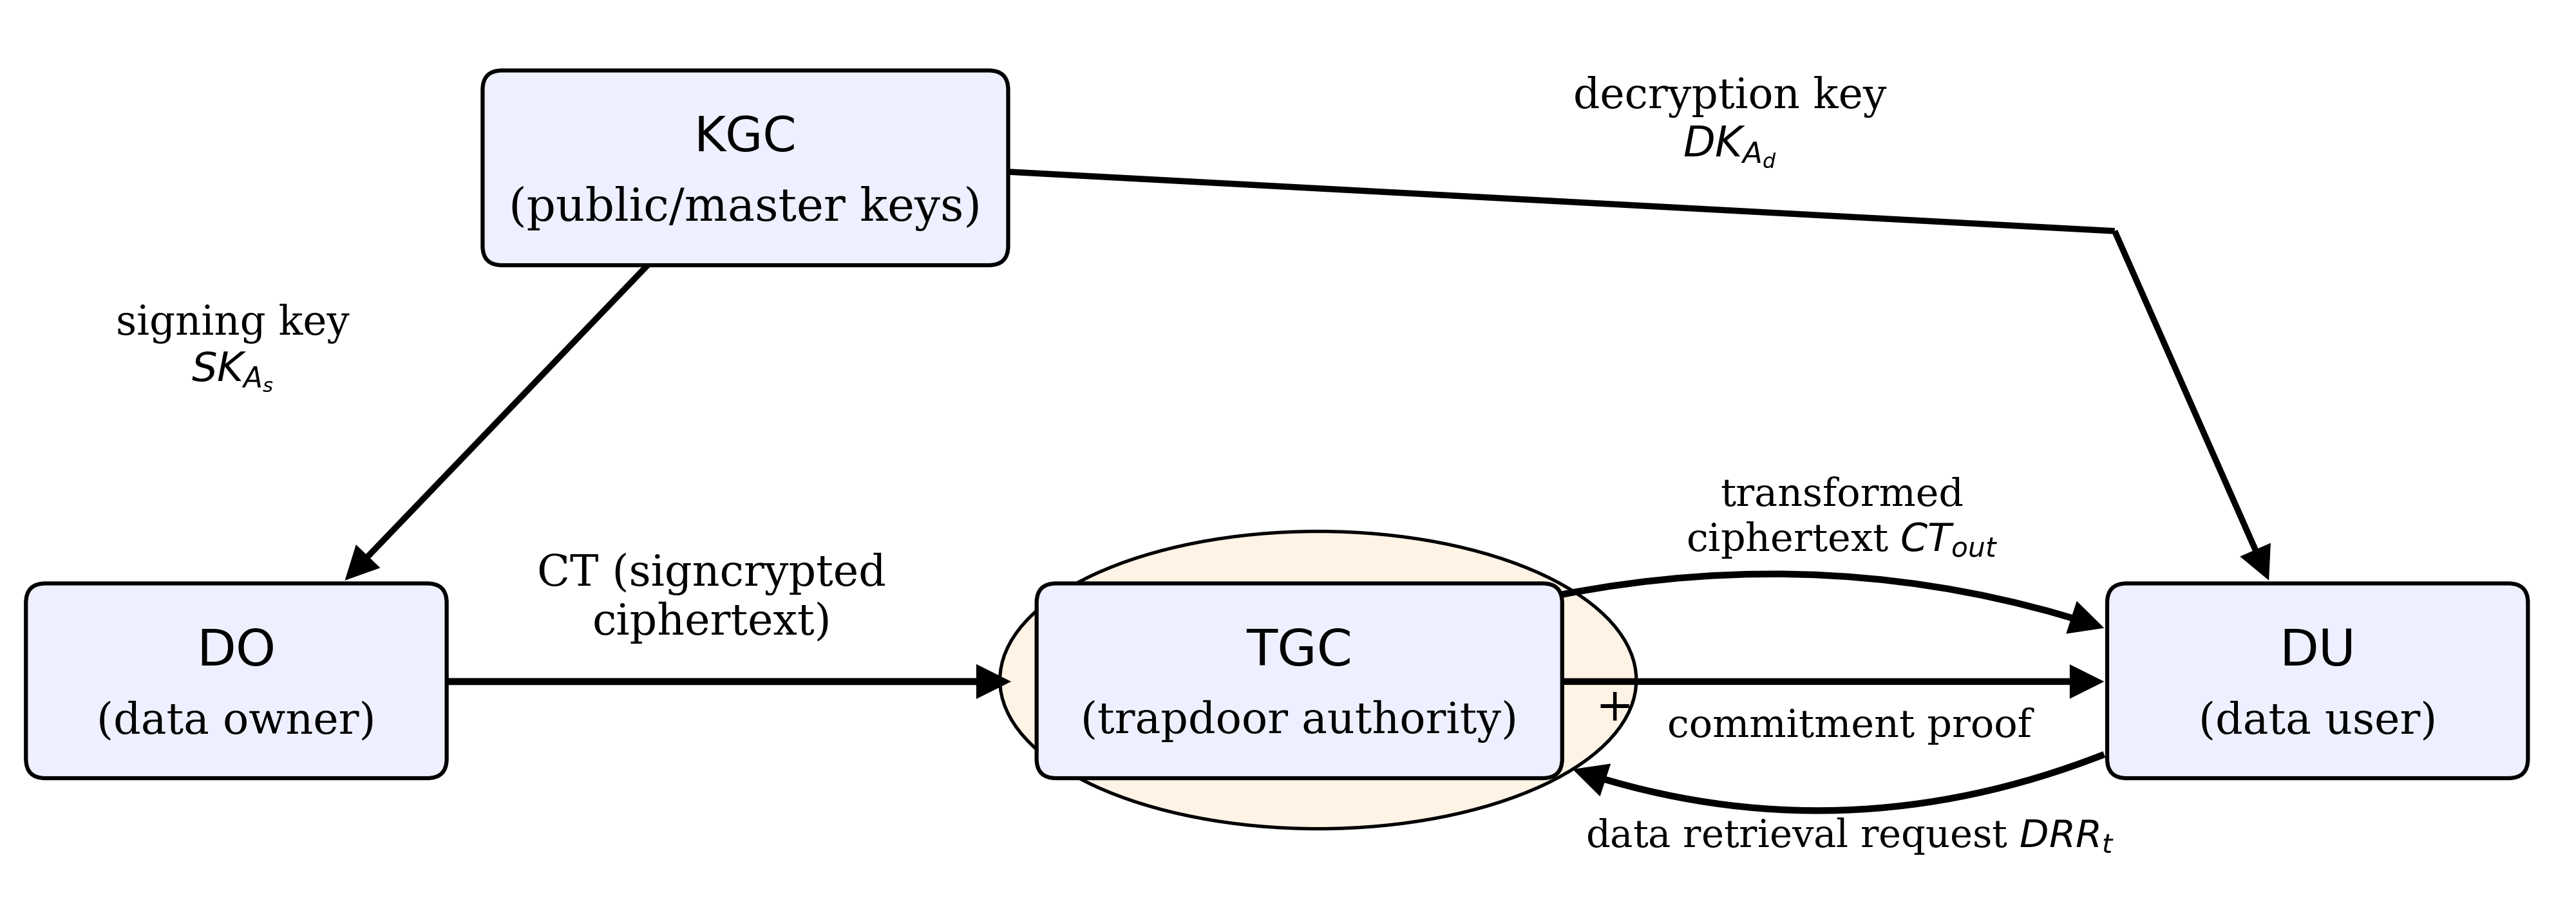
\includegraphics[width=\textwidth]{Figures/architecture.png}
\caption{System architecture and message flow of PQ-ABDSRS. The entity roles and message
flow follow ABDSRS; every pairing operation at each edge is replaced by a lattice operation.
$\KGC$ is the key generation center, $\TGC$ the trapdoor generation center, $\DO$ a data
owner, $\DU$ a data user and $\CS$ the cloud server.}
\label{fig:architecture}
\end{figure}

\begin{table}[htbp]
\centering
\caption{Notation used in the construction.}
\label{tab:notation}
\begin{tabularx}{\textwidth}{lL}
\toprule
Symbol & Meaning \\
\midrule
$\KGC$, $\TGC$ & key generation center, trapdoor generation center \\
$\DO$, $\DU$, $\CS$ & data owner, data user, cloud server \\
$\PP$, $\MK$ & system public parameters, master secret key \\
$U$, $U^{\circ}$ & attribute universe, keyword-name universe \\
$A_s$, $A_d$ & signing attribute set, decryption attribute set \\
$\SK_{A_s}$, $\DK_{A_d}$ & signing key ($\ABS$), decryption key ($\CPABE$) \\
$\mathcal{P}_e,\mathcal{P}_s,\mathcal{P}_t$ & encryption, signing, keyword policy \\
$S_1,\dots,S_{\ell_e}$ & DNF clauses of $\mathcal{P}_e$, per~\eqref{eq:dnf} \\
$W$, $W^{\circ}$ & keyword value set, keyword generic-name set, $|W|=|W^{\circ}|=\varsigma$ \\
$\mathsf{ct}_j$, $\mathsf{ct}_W$ & $\CPABE$ ciphertext of clause $S_j$, $\KPABE$ ciphertext of $W^{\circ}$ \\
$\mathbf{d}_j$, $\mu_{\mathrm{sig}}$ & binding digest of $\mathsf{ct}_j$, $\ABS$ signature \\
$\CT$, $\CT_{\mathrm{out}}$ & stored ciphertext, transformed ciphertext \\
$\DRR$ & data retrieval request \\
$\TD_{\mathcal{P}_t}$ & keyword-policy trapdoor \\
$K$, $\tau$ & encapsulated payload key, search tag preimage, both in $\bt^{\kappa}$ \\
$\mathbf{A}_h$ & digest matrix of Definition~\ref{def:digest} \\
$\hSIS(\cdot)$ & SIS-based binding digest \\
$\CPABE,\KPABE,\ABS$ & building blocks of Definitions~\ref{def:cpabe},~\ref{def:kpabe},~\ref{def:abs} \\
$n,q,m,\sigma,\alpha$ & lattice dimension, modulus, matrix width, Gaussian parameter, error rate \\
$\beta_s$, $\beta_h$ & SIS norm bounds of the signature and the digest (Table~\ref{tab:coresvp}) \\
$B_{\mathrm{abe}}$ & $\CPABE$ decryption-error bound (Definition~\ref{def:babe}) \\
$h$ & $\lceil\log_2 q\rceil$ \\
\bottomrule
\end{tabularx}
\end{table}

\subsection{Entity roles}

$\KGC$ runs the setup of the three building blocks (Section~\ref{sec:blocks}) and issues
signing keys to $\DO$s and decryption keys to $\DU$s through $\ABS.\KeyGen$ and
$\CPABE.\KeyGen$; under the dimension model of Remark~\ref{rem:dimmodel} these rest on lattice
trapdoor generation and preimage sampling over delegated bases
(Definitions~\ref{def:trapgen}--\ref{def:extbasis}).
$\DO$ signcrypts data under a signing policy $\mathcal{P}_s$, an encryption policy
$\mathcal{P}_e$ and a keyword set $W$, and uploads the result to $\CS$.
$\CS$ stores signcrypted data and, on receiving a $\DRR$, executes $\Test$ and $\Transform$,
returning a transformed ciphertext with the evidence needed for verification.
$\TGC$ issues keyword-policy trapdoors to $\DU$s.
$\DU$ obtains a trapdoor from $\TGC$, sends a $\DRR$ to $\CS$, and runs $\USV$ on the reply.

\subsection{Threat model}
\label{subsec:threat}

$\KGC$ and $\TGC$ are fully trusted. The cloud is modeled as \emph{malicious} with the
following permitted deviations, replacing the contradictory
``honest-but-potentially-malicious'' formulation of the earlier version. $\CS$ stores what it
is given, but it may (i) attempt to learn plaintexts, keyword values or attribute sets from
the data it holds; (ii) return a ciphertext other than the one the $\DRR$ selects, or a
ciphertext from a different record; (iii) skip the $\Test$ evaluation and claim a match or a
non-match; (iv) skip signature verification; and (v) collude with any set of $\DU$s. $\CS$
may not modify or delete stored records without detection, which is the standard availability
assumption of this line of work and is orthogonal to the properties proved here. We state
explicitly that a negative search result is not verifiable: a cloud that claims no record
matches cannot be contradicted non-interactively, and the same holds in
ABDSRS~\cite{bera2023designing}.

$\DU$s are untrusted and may attempt to unsigncrypt ciphertexts they are not authorized for,
collude beyond their combined access rights, or attempt to learn keyword values. $\DO$s may
attempt to upload ciphertexts signed under policies they do not satisfy. In addition,
adversaries are allowed to be QPT with respect to the hardness assumptions of
Section~\ref{subsec:hardproblems}, but only classical access to the random oracles is
modeled (Section~\ref{subsec:scope}).

%=================================================================
\section{Construction of PQ-ABDSRS}
\label{sec:construction}

PQ-ABDSRS has the seven phases of ABDSRS: system initialization, key generation,
signcryption, keyword-policy trapdoor generation, data retrieval request generation, data
retrieval ($\Test$ and $\Transform$), and unsigncryption with verification. Every algorithm
below states the type of each input and output.

\subsection{System initialization}

\begin{algorithm}[htbp]
\caption{$\Setup(1^{\lambda}, U, U^{\circ})$}
\label{alg:setup}
\begin{algorithmic}[1]
\Require security parameter $1^{\lambda}$, attribute universe $U$, keyword-name universe $U^{\circ}$
\Ensure public parameters $\PP$, master secret key $\MK$
\State Fix $n,q,\alpha,\sigma,\kappa$ per Section~\ref{subsec:params}; set $h := \lceil\log_2 q\rceil$, $m := 2nh$, $\chi := D_{\Z,\alpha q}$
\State $(\mathsf{pp}_{\mathrm{cp}},\mathsf{msk}_{\mathrm{cp}}) \leftarrow \CPABE.\Setup(1^{\lambda},U)$ \Comment{Def.~\ref{def:cpabe}; dimensions per Rem.~\ref{rem:dimmodel}}
\State $(\mathsf{pp}_{\mathrm{kp}},\mathsf{msk}_{\mathrm{kp}}) \leftarrow \KPABE.\Setup(1^{\lambda},U^{\circ})$ \Comment{Def.~\ref{def:kpabe}}
\State $(\mathsf{pp}_{\mathrm{abs}},\mathsf{msk}_{\mathrm{abs}}) \leftarrow \ABS.\Setup(1^{\lambda},U)$ \Comment{Def.~\ref{def:abs}}
\State $\mathbf{A}_h \xleftarrow{\$} \Zq^{n \times 2nh}$ \Comment{digest matrix, Def.~\ref{def:digest}}
\State Select hash functions, modeled as independent random oracles:
\Statex \quad $H_1 : \bt^{*} \to \Zq^{n\times m}$ \Comment{seed expansion, Rem.~\ref{rem:seeds}}
\Statex \quad $H_2 : \bt^{\kappa} \to \bt^{\kappa}$ \Comment{payload key derivation}
\Statex \quad $H_3 : \bt^{*} \to \Zq^{n}$ \Comment{message-to-target for $\ABS$}
\Statex \quad $H_4 : \bt^{\kappa} \to \bt^{\kappa}$ \Comment{search-tag function}
\State $\PP := \big(n,q,m,h,\sigma,\alpha,\kappa,\ \mathsf{pp}_{\mathrm{cp}},\mathsf{pp}_{\mathrm{kp}},\mathsf{pp}_{\mathrm{abs}},\ \mathbf{A}_h,\ H_1,\dots,H_4\big)$
\State $\MK := \big(\mathsf{msk}_{\mathrm{cp}},\ \mathsf{msk}_{\mathrm{kp}},\ \mathsf{msk}_{\mathrm{abs}}\big)$
\State \Return $(\PP,\MK)$
\end{algorithmic}
\end{algorithm}

Algorithm~\ref{alg:setup} is the lattice analogue of ABDSRS's $\KGC$ setup: the pairing tuple
$\langle p,\mathbb{G},\mathbb{G}_T,e\rangle$ with generators $g,g_1,\dots,g_{15}$
(Section 4.1 of~\cite{bera2023designing}) is replaced by the three lattice building blocks and
the digest matrix $\mathbf{A}_h$. Under the dimension model of Remark~\ref{rem:dimmodel} the
access-control layer contributes one matrix in $\Zq^{n\times m}$ per attribute, and the
keyword layer one per keyword name, so $\PP$ holds $2|U|+3$ such matrices when
$|U^{\circ}| = |U|$. This is the dominant cost in Section~\ref{sec:performance}, and
Remark~\ref{rem:seeds} discusses seed derivation via $H_1$.

\begin{Remark}[Seed derivation of public matrices]
\label{rem:seeds}
Every uniform public matrix, in both the access-control and the keyword layer, may be defined
as $H_1(\mathsf{seed}\Vert\,\text{index})$ for a single $256$-bit public seed, as is standard
in lattice KEM and signature standards. This reduces the \emph{transmitted} public parameters
to $32(2|U|+4)$ bytes when $|U^{\circ}| = |U|$, counting one seed per derivable matrix and one
for the target matrix $\mathbf{U}$. It does not reduce the working memory or the arithmetic
cost, since every matrix must be expanded before use.
Table~\ref{tab:concrete} reports both figures, and neither is presented as though it were the
other.
\end{Remark}

\subsection{Key generation}

\begin{algorithm}[htbp]
\caption{$\KeyGen(\PP,\MK,A,\mathsf{mode})$}
\label{alg:keygen}
\begin{algorithmic}[1]
\Require attribute set $A\subseteq U$, $\mathsf{mode}\in\{\mathsf{dec},\mathsf{sign}\}$
\Ensure decryption key $\DK_{A}$ or signing key $\SK_{A}$
\If{$\mathsf{mode} = \mathsf{dec}$}
    \State $\mathsf{sk}^{\mathrm{cp}}_{A} \leftarrow \CPABE.\KeyGen(\mathsf{msk}_{\mathrm{cp}},A)$ \Comment{Def.~\ref{def:cpabe}; a matrix in $\Z^{2m\times\kappa}$ under Rem.~\ref{rem:dimmodel}}
    \State \Return $\DK_{A} := (A,\mathsf{sk}^{\mathrm{cp}}_{A})$
\Else
    \State $\mathsf{sk}^{\mathrm{abs}}_{A} \leftarrow \ABS.\KeyGen(\mathsf{msk}_{\mathrm{abs}},A)$ \Comment{Def.~\ref{def:abs}}
    \State \Return $\SK_{A} := (A,\mathsf{sk}^{\mathrm{abs}}_{A})$
\EndIf
\end{algorithmic}
\end{algorithm}

Neither branch of Algorithm~\ref{alg:keygen} opens its building block. Two errors in earlier
versions are removed by this: a width-$m$ preimage was counted against a width-$2m$ matrix,
and a single preimage vector was used where $\kappa$ independent targets are required
(Remark~\ref{rem:dimmodel}). All sizes in Section~\ref{sec:performance} use a key of
dimension $2m\times\kappa$.

\subsection{Attribute-based online/offline signcryption}
\label{subsec:signcrypt}

\begin{algorithm}[htbp]
\caption{$\OffSC(\PP,\ell_{\max})$}
\label{alg:offsigncrypt}
\begin{algorithmic}[1]
\Require bound $\ell_{\max}$ on the number of DNF clauses
\Ensure message-independent intermediate ciphertext $\mathsf{IC}$
\State $K \xleftarrow{\$} \bt^{\kappa}$, \; $\tau \xleftarrow{\$} \bt^{\kappa}$ \Comment{payload key and search-tag preimage}
\For{$j \in [\ell_{\max}]$}
    \State $r_j \xleftarrow{\$} \mathcal{R}_{\mathrm{cp}}$ \Comment{randomness for one $\CPABE.\Enc$ invocation}
\EndFor
\State $r_{\mathrm{kp}} \xleftarrow{\$} \mathcal{R}_{\mathrm{kp}}$ \Comment{randomness for $\KPABE.\Enc$}
\State $\mathsf{nc} \xleftarrow{\$} \bt^{96}$ \Comment{AEAD nonce}
\State \Return $\mathsf{IC} := (K,\tau,\{r_j\}_{j\in[\ell_{\max}]},r_{\mathrm{kp}},\mathsf{nc})$
\end{algorithmic}
\end{algorithm}

\begin{algorithm}[htbp]
\caption{$\OnSC(\PP,\SK_{A_s},\mathsf{IC},\mathit{msg},\mathcal{P}_e,\mathcal{P}_s,W)$}
\label{alg:onsigncrypt}
\begin{algorithmic}[1]
\Require message $\mathit{msg}\in\bt^{*}$, encryption policy $\mathcal{P}_e$ with DNF clauses $S_1,\dots,S_{\ell_e}$, signing policy $\mathcal{P}_s$, keyword set $W$ with generic names $W^{\circ}$
\Ensure ciphertext $\CT$, or $\bot$
\State \textbf{if} $\mathcal{P}_s(A_s) = \false$ \textbf{then return} $\bot$ \Comment{explicit signing-policy check}
\For{$j \in [\ell_e]$} \Comment{one $\CPABE$ ciphertext per DNF clause, same payload $K$}
    \State $\mathsf{ct}_j := \CPABE.\Enc(\mathsf{pp}_{\mathrm{cp}},S_j,K;\,r_j)$
    \State $\mathbf{d}_j := \hSIS(\mathsf{ct}_j) \in \Zq^{n}$ \Comment{binding digest over the serialization, Def.~\ref{def:digest}}
\EndFor
\State $\mathsf{ct}_W := \KPABE.\Enc(\mathsf{pp}_{\mathrm{kp}},W^{\circ},\tau;\,r_{\mathrm{kp}})$ \Comment{keyword layer, Section~\ref{subsec:keywords}}
\State $\mathsf{tag} := H_4(\tau) \in \bt^{\kappa}$ \Comment{public match target}
\State $k := H_2(K)$
\State $\mathsf{hdr} := \big(\mathcal{P}_e \Vert \mathcal{P}_s \Vert W^{\circ} \Vert \mathsf{tag} \Vert \{\mathbf{d}_j\}_{j\in[\ell_e]}\big)$
\State $c_{\mathrm{dem}} \leftarrow \AEAD.\Enc(k,\mathsf{nc},\mathsf{hdr},\mathit{msg})$ \Comment{KEM--DEM, Section~\ref{subsec:aead}}
\State $\mu_{\mathrm{sig}} \leftarrow \ABS.\Sign\big(\mathsf{sk}^{\mathrm{abs}}_{A_s},\mathcal{P}_s,\ H_3(\mathsf{hdr}\Vert \mathsf{nc} \Vert c_{\mathrm{dem}})\big)$
\State \Return $\CT := \big(\mathcal{P}_e,\mathcal{P}_s,W^{\circ},\{\mathsf{ct}_j\}_{j\in[\ell_e]},\{\mathbf{d}_j\}_{j\in[\ell_e]},\mathsf{ct}_W,\mathsf{tag},\mathsf{nc},c_{\mathrm{dem}},\mu_{\mathrm{sig}}\big)$
\end{algorithmic}
\end{algorithm}

Four points are worth naming. First, the payload is no longer a one-time pad
$\mathit{msg}\oplus H(\cdot)$, which is defined only for a fixed-length bit string and
provides no integrity; it is an AEAD ciphertext under a key encapsulated by the
attribute-based layer. Second, the digests $\{\mathbf{d}_j\}$ are inside the signed header,
which is what binds the stored ciphertext components to the data owner. Third, the
signing-policy check $\mathcal{P}_s(A_s)=\true$ is explicit, and $\ABS.\Sign$ proves that it
holds without revealing $A_s$ (Definition~\ref{def:abs}). Fourth, the $\ell_e$ clause
ciphertexts are independent invocations of $\CPABE.\Enc$ on a common payload $K$; they do not
share a secret, and the hybrid over them is what contributes the factor $\ell_e$ to
Theorem~\ref{thm:confidentiality}. The online/offline split is preserved: $K$, $\tau$, the
per-invocation randomness and the nonce are message-independent and are drawn in
Algorithm~\ref{alg:offsigncrypt}.

\subsection{Keyword layer and trapdoor generation}
\label{subsec:keywords}

As in ABDSRS, only \emph{generic names} of keywords appear in ciphertexts and policies. The
$\DO$ and authorized $\DU$s share the mapping from generic names to keyword values out of
band; the cloud sees $W^{\circ}$ and $\mathcal{P}_t$ over $U^{\circ}$ but never the values.
This is a representation-level mechanism, not an algebraic one, and it is retained unchanged.
We state precisely what it gives: the cloud learns which generic names occur and whether a
queried policy matches, and it does not learn the keyword values. It is not attribute-hiding
in the cryptographic sense, and we do not claim that it is.

\begin{algorithm}[htbp]
\caption{$\KTG(\PP,\MK,\mathcal{P}_t)$}
\label{alg:kwtrapgen}
\begin{algorithmic}[1]
\Require keyword policy $\mathcal{P}_t$, a monotone Boolean formula over $U^{\circ}$
\Ensure keyword trapdoor $\TD_{\mathcal{P}_t}$
\State $\mathsf{sk}_{\mathcal{P}_t} \leftarrow \KPABE.\KeyGen(\mathsf{msk}_{\mathrm{kp}},\mathcal{P}_t)$
\State \Return $\TD_{\mathcal{P}_t} := (\mathcal{P}_t,\ \mathsf{sk}_{\mathcal{P}_t})$
\end{algorithmic}
\end{algorithm}

\begin{algorithm}[htbp]
\caption{$\DRRGen(\PP,\DK_{A_d},\TD_{\mathcal{P}_t},\mathcal{P}_e)$}
\label{alg:drr}
\begin{algorithmic}[1]
\Require attribute set $A_d$ from $\DK_{A_d}$, keyword trapdoor $\TD_{\mathcal{P}_t} = (\mathcal{P}_t,\mathsf{sk}_{\mathcal{P}_t})$, target encryption policy $\mathcal{P}_e$
\Ensure data retrieval request $\DRR$
\State $j^{\ast} := \mathsf{Idx}(\mathcal{P}_e,A_d)$ \Comment{Section~\ref{subsec:policyclass}}
\State \textbf{if} $j^{\ast} = \bot$ \textbf{then return} $\bot$
\State \Return $\DRR := (\mathcal{P}_t,\ \mathsf{sk}_{\mathcal{P}_t},\ j^{\ast})$
\end{algorithmic}
\end{algorithm}

The $\DRR$ contains the clause index $j^{\ast}$ rather than a blinded transform key. This is
a deliberate departure from ABDSRS, and it has a cost that we state rather than hide: the
cloud learns which DNF clause the $\DU$'s attribute set satisfies. It does not learn $A_d$
itself, and it receives no part of $\mathsf{sk}^{\mathrm{cp}}_{A_d}$. In ABDSRS the cloud
receives a blinded transform key derived from the user's key rather than the key itself, so
the difference is that PQ-ABDSRS transmits no key material at all, not that ABDSRS exposes a
key.

\subsection{Data retrieval}
\label{subsec:testtransform}

Data retrieval is two algorithms run by $\CS$ on a stored record. $\Test$ decides whether the
record matches the keyword policy of the request and, when it does, returns the preimage
$\tau'$ that the $\DU$ will check against the signed $\mathsf{tag}$. $\Transform$ then selects
the one clause ciphertext the $\DU$ can decrypt and assembles the reply. Neither algorithm
holds a secret of its own: $\CS$ acts only on the trapdoor supplied in the $\DRR$ and on
public data, which is why a dishonest execution is detectable by
Section~\ref{subsec:verifmech} rather than preventable.

\begin{algorithm}[htbp]
\caption{$\Test(\PP,\CT,\DRR)$}
\label{alg:test}
\begin{algorithmic}[1]
\Require stored ciphertext $\CT$, request $\DRR = (\mathcal{P}_t,\mathsf{sk}_{\mathcal{P}_t},j^{\ast})$
\Ensure $(\mathsf{match},\tau')$ or $\bot$
\State Parse $\CT$ for $\mathsf{ct}_W$ and $\mathsf{tag}$
\State $\tau' \leftarrow \KPABE.\Dec(\mathsf{sk}_{\mathcal{P}_t},\mathsf{ct}_W)$
\State \textbf{if} $\tau' = \bot$ \textbf{or} $H_4(\tau') \ne \mathsf{tag}$ \textbf{then return} $\bot$
\State \Return $(\mathsf{match},\tau')$ \Comment{$\tau'$ is the cloud's evidence of a genuine match}
\end{algorithmic}
\end{algorithm}

\begin{algorithm}[htbp]
\caption{$\Transform(\PP,\CT,\DRR)$}
\label{alg:transform}
\begin{algorithmic}[1]
\Require stored ciphertext $\CT$, request $\DRR$
\Ensure transformed ciphertext $\CT_{\mathrm{out}}$ or $\bot$
\State Parse $\CT$ for $\mathcal{P}_e$ (hence $\ell_e$) and $\{\mathsf{ct}_j\}_{j\in[\ell_e]}$; parse $\DRR$ for $j^{\ast}$
\State $\rho \leftarrow \Test(\PP,\CT,\DRR)$; \textbf{if} $\rho = \bot$ \textbf{then return} $\bot$; \textbf{else} parse $\rho = (\mathsf{match},\tau')$
\State \textbf{if} $j^{\ast} \notin [\ell_e]$ \textbf{then return} $\bot$
\State $\mathsf{ct}_{\mathrm{out}} := \CPABE.\mathsf{Select}(\{\mathsf{ct}_j\}_{j\in[\ell_e]},j^{\ast}) = \mathsf{ct}_{j^{\ast}}$ \Comment{Definition~\ref{def:cpabe}}
\State \Return $\CT_{\mathrm{out}} := \big(j^{\ast},\mathsf{ct}_{\mathrm{out}},\tau',\mathcal{P}_e,\mathcal{P}_s,W^{\circ},\{\mathbf{d}_j\}_{j\in[\ell_e]},\mathsf{tag},\mathsf{nc},c_{\mathrm{dem}},\mu_{\mathrm{sig}}\big)$
\end{algorithmic}
\end{algorithm}

\subsection{The verifiability mechanism}
\label{subsec:verifmech}

ABDSRS verifies the cloud implicitly: a cheating cloud cannot produce values satisfying the
pairing identity $X_1X_2 = k_T^{\mathsf{H}(\mathsf{ot})}$, in the notation of that paper,
without knowing a discrete logarithm
(Remark 6 of~\cite{bera2023designing}). There is no lattice identity with that property, and
by Remark~\ref{rem:commitment-insufficient} a homomorphic commitment does not substitute for
one. PQ-ABDSRS instead makes the check explicit and splits it in two.

\emph{Correctness of $\Transform$.} The $\DO$ signs the digest list $\{\mathbf{d}_j\}$ inside
$\mathsf{hdr}$. The $\DU$ receives $\mathsf{ct}_{\mathrm{out}}$ and $j^{\ast}$, recomputes
$\hSIS(\mathsf{ct}_{\mathrm{out}})$ and compares it with $\mathbf{d}_{j^{\ast}}$, having first
verified $\mu_{\mathrm{sig}}$ over the header that contains the digests. A cloud that
returns anything other than the genuine $\mathsf{ct}_{j^{\ast}}$ must therefore either find a digest collision or forge a $\ABS$ signature. This is the authenticated relation between the
stored object, the applied function and the output that Remark~\ref{rem:commitment-insufficient}
identifies as missing.

\emph{Correctness of $\Test$.} The cloud returns $\tau'$, and the $\DU$ checks
$H_4(\tau') = \mathsf{tag}$ against the signed $\mathsf{tag}$. A cloud that did not actually
decrypt $\mathsf{ct}_W$ under a satisfying trapdoor must invert $H_4$ on a target it did not
choose.

\subsection{Unsigncryption and verification}
\label{subsec:unsigncrypt}

\begin{algorithm}[htbp]
\caption{$\USV(\PP,\DK_{A_d},\CT_{\mathrm{out}})$}
\label{alg:unsigncrypt}
\begin{algorithmic}[1]
\Require decryption key $\DK_{A_d} = (A_d,\mathsf{sk}^{\mathrm{cp}}_{A_d})$, transformed ciphertext
\Ensure $\mathit{msg}$ or $\bot$
\State Parse $\CT_{\mathrm{out}}$; set $\mathsf{hdr} := (\mathcal{P}_e\Vert\mathcal{P}_s\Vert W^{\circ}\Vert\mathsf{tag}\Vert\{\mathbf{d}_j\})$
\State \textbf{if} $\ABS.\Verify(\mathsf{pp}_{\mathrm{abs}},\mathcal{P}_s,H_3(\mathsf{hdr}\Vert\mathsf{nc}\Vert c_{\mathrm{dem}}),\mu_{\mathrm{sig}}) = \mathsf{reject}$ \textbf{then return} $\bot$
\State \textbf{if} $H_4(\tau') \ne \mathsf{tag}$ \textbf{then return} $\bot$ \Comment{$\Test$ was not executed honestly}
\State \textbf{if} $\hSIS(\mathsf{ct}_{\mathrm{out}}) \ne \mathbf{d}_{j^{\ast}}$ \textbf{then return} $\bot$ \Comment{$\Transform$ was not executed honestly}
\State \textbf{if} $S_{j^{\ast}} \not\subseteq A_d$ \textbf{then return} $\bot$
\State $K' \leftarrow \CPABE.\Dec(\mathsf{sk}^{\mathrm{cp}}_{A_d},\mathsf{ct}_{\mathrm{out}})$; \textbf{if} $K' = \bot$ \textbf{then return} $\bot$
\State $\mathit{msg} \leftarrow \AEAD.\Dec(H_2(K'),\mathsf{nc},\mathsf{hdr},c_{\mathrm{dem}})$
\State \Return $\mathit{msg}$ \Comment{$\AEAD.\Dec$ returns $\bot$ on tag failure}
\end{algorithmic}
\end{algorithm}

Every value used in lines 2 to 5 of Algorithm~\ref{alg:unsigncrypt} is present in
$\CT_{\mathrm{out}}$ or in $\PP$; in particular the policies, keyword names and digests are
carried in the transformed ciphertext precisely because signature verification requires them.
The earlier version omitted them from $\CT_{\mathrm{out}}$, which made verification
impossible as written, and omitted them from the size accounting.

%=================================================================
\section{Correctness}
\label{sec:correctness}

\begin{Definition}[Decryption-error bound of $\CPABE$]
\label{def:babe}
$\CPABE$ has decryption-error bound $B_{\mathrm{abe}}$ at modulus $q$ if, for every clause $S$,
every $A\supseteq S$ and every $K\in\bt^{\kappa}$, honest execution of
$\CPABE.\Dec(\mathsf{sk}_A,\CPABE.\Enc(\mathsf{pp},S,K))$ recovers $K$ whenever the additive
error accumulated in each payload coordinate is at most $B_{\mathrm{abe}} < q/4$.
\end{Definition}

Under the dimension model of Remark~\ref{rem:dimmodel} the error in one payload coordinate is
$\inner{\mathbf{e}_{A}}{\mathbf{e}_{S}} + e$, where $\mathbf{e}_{A}$ is the corresponding
column of the key matrix, $\mathbf{e}_{S}$ is the ciphertext noise and $e$ is the
encapsulation noise in that coordinate. Taking a union bound over the $\kappa$ payload
coordinates, so that the tail factor is $\omega(\sqrt{\log\kappa})$ rather than the
$\omega(\sqrt{\log m})$ of Definition~\ref{def:gaussian}, gives
\begin{equation}
\label{eq:noise}
B_{\mathrm{abe}} \;=\; \big(\sigma\sqrt{2m} + 1\big)\cdot\alpha q\cdot\omega(\sqrt{\log \kappa})
\;<\; \frac{q}{4} .
\end{equation}
Section~\ref{subsec:params} fixes $q$ from~\eqref{eq:noise}. Any instantiation whose own error
bound differs must substitute it here; the expression is the bound for the inner-product
decryption common to the dual-Regev family, not a figure taken from~\cite{zhang2012ciphertext}.

\begin{Theorem}[Correctness]
\label{thm:correctness}
Let $\mathcal{P}_e$ have DNF clauses $S_1,\dots,S_{\ell_e}$ and let $A_d$ satisfy
$\mathcal{P}_e$ with $j^{\ast} = \mathsf{Idx}(\mathcal{P}_e,A_d)$, so $S_{j^{\ast}} \subseteq A_d$.
Suppose all parties are honest, $\CPABE$ and $\KPABE$ are correct in the sense of
Definitions~\ref{def:cpabe} and~\ref{def:kpabe}, $\CPABE$ satisfies~\eqref{eq:noise}, and
$\AEAD$ is correct. Then
$\USV(\PP,\DK_{A_d},\Transform(\PP,\CT,\DRR)) = \mathit{msg}$ with probability at least
$1-\negl(\lambda)$.
\end{Theorem}

\begin{proof}
Honest execution of $\Test$ gives $\tau' = \tau$ by correctness of $\KPABE$, since
$\mathcal{P}_t(W^{\circ}) = \true$, so line 3 of Algorithm~\ref{alg:unsigncrypt} accepts.
Honest execution of $\Transform$ gives
$\mathsf{ct}_{\mathrm{out}} = \mathsf{ct}_{j^{\ast}}$, so
$\hSIS(\mathsf{ct}_{\mathrm{out}}) = \mathbf{d}_{j^{\ast}}$ and line 4 accepts; line 2 accepts
because the header is the one the $\DO$ signed, and line 5 because
$S_{j^{\ast}}\subseteq A_d$. Line 6 therefore invokes $\CPABE.\Dec$ on a ciphertext for a
clause contained in $A_d$, which returns $K' = K$ except with probability $\negl(\lambda)$ by
correctness of $\CPABE$ under~\eqref{eq:noise}. Hence $H_2(K') = H_2(K) = k$, and
$\AEAD.\Dec$ with the correct key, nonce and associated data returns $\mathit{msg}$.
\end{proof}

The scheme adds no noise of its own: $\hSIS$ is exact, the $\AEAD$ layer is exact, and the
random-oracle checks are exact. All decryption error lives inside $\CPABE$, which is why
Definition~\ref{def:babe} isolates it. Under~\eqref{eq:noise}, with the parameters of
Section~\ref{subsec:params} and $\omega(\sqrt{\log\kappa})$ instantiated by the constant $5$,
the left-hand side is $2^{24.1}$ against $q/4 = 2^{28}$, leaving $2^{3.9}$ of margin. The bound
involves a single clause, since decryption uses exactly one $\mathsf{ct}_{j^{\ast}}$, so it does
not grow with $\ell_e$.

%=================================================================
\section{Security Analysis}
\label{sec:security}

We establish data confidentiality, data unforgeability, verifiability, signer privacy and
keyword indistinguishability. Every proof is in the classical random oracle model. Where a
statement follows from a building-block property rather than from a new reduction,
Table~\ref{tab:inherited} records which one, and the proof says so explicitly.

\subsection{Data confidentiality}

Following ABDSRS's two-adversary split (Section 3.5.1 of~\cite{bera2023designing}), a
\emph{Type-1} adversary is a malicious cloud or an unauthorized $\DU$, and a \emph{Type-2}
adversary is an authorized $\DU$ that does not hold the trapdoor for the challenge keyword
policy. Since PQ-ABDSRS gives the cloud no secret key at all, the distinction reduces to
which oracles are available.

\begin{Definition}[Selective IND-CPA game for PQ-ABDSRS]
\label{def:indcpa}
The challenger $\Chal$ and adversary $\Adv$ interact as follows.
\begin{enumerate}[leftmargin=*,itemsep=1pt]
    \item $\Adv$ outputs a challenge encryption policy $\mathcal{P}_e^{\star}$ with DNF clauses
          $S_1^{\star},\dots,S_{\ell}^{\star}$, where $\ell$ denotes their number, a challenge
          keyword set $W^{\star}$, and a signing policy $\mathcal{P}_s$ together with an
          attribute set $A_s$ satisfying it, under which the challenge will be signed.
    \item $\Chal$ runs $\Setup(1^{\lambda},U,U^{\circ})\to(\PP,\MK)$ and gives $\PP$ to
          $\Adv$.
    \item $\Adv$ adaptively queries: $\mathcal{O}_{\KeyGen}(A_d)$, answered for any $A_d$
          with $\mathcal{P}_e^{\star}(A_d) = \false$; $\mathcal{O}_{\Sign}(A_s)$ for signing
          keys, answered for all $A_s$; $\mathcal{O}_{\mathsf{SC}}$ for signcryptions of
          arbitrary $(\mathit{msg},\mathcal{P}_s,\mathcal{P}_e,W)$; and
          $\mathcal{O}_{\KTG}(\mathcal{P}_t)$, answered for any $\mathcal{P}_t$ with
          $\mathcal{P}_t(W^{\star\circ}) = \false$.
    \item $\Adv$ outputs $\mathit{msg}_0^{\star},\mathit{msg}_1^{\star}$ of equal length.
    \item $\Chal$ samples $b\xleftarrow{\$}\bt$ and returns
          $\CT^{\star} \leftarrow \OnSC(\PP,\SK_{A_s},\mathsf{IC},\mathit{msg}_b^{\star},\mathcal{P}_e^{\star},\mathcal{P}_s,W^{\star})$.
    \item $\Adv$ repeats step 3 under the same restrictions and outputs $b'$.
\end{enumerate}
$\Adv$ wins if $b'=b$, and
$\mathsf{Adv}^{\mathsf{IND\text{-}CPA}}_{\Adv}(\lambda) := |\Pr[b'=b] - 1/2|$.
A \emph{Type-1} adversary is additionally denied $\mathcal{O}_{\KTG}$ on every policy; a
\emph{Type-2} adversary may query it under the restriction stated in step 3.
\end{Definition}

\begin{Theorem}[Data confidentiality]
\label{thm:confidentiality}
If $\CPABE$ is selectively IND-CPA secure under $\LWE_{n,q,\chi,m}$, $\AEAD$ is IND-CPA
secure, and $H_2$ is a random oracle, then for every PPT adversary $\Adv$ of either type,
$\mathsf{Adv}^{\mathsf{IND\text{-}CPA}}_{\Adv}(\lambda) \le
\ell\cdot\mathsf{Adv}^{\CPABE}_{\Chal}(\lambda) + \mathsf{Adv}^{\AEAD}_{\Chal}(\lambda) +
q_H\cdot 2^{-\kappa}$, where $\ell$ is the number of clauses of $\mathcal{P}_e^{\star}$ and
$q_H$ bounds the number of $H_2$ queries.
\end{Theorem}

\begin{proof}
We proceed by a hybrid over the clauses followed by two game hops. $\mathsf{G}_0$ is
Definition~\ref{def:indcpa}. For $t\in\{0,\dots,\ell\}$ let $\mathsf{H}_t$ be $\mathsf{G}_0$
with the first $t$ clause ciphertexts $\mathsf{ct}_1^{\star},\dots,\mathsf{ct}_t^{\star}$
replaced by encryptions of an independent uniform
$\widetilde{K}\xleftarrow{\$}\bt^{\kappa}$; thus $\mathsf{H}_0 = \mathsf{G}_0$ and
$\mathsf{H}_{\ell} =: \mathsf{G}_1$. The hybrid is needed because the $\ell$ clause
ciphertexts are separate invocations of $\CPABE.\Enc$ on a common payload, whereas
Definition~\ref{def:cpabe} gives indistinguishability for one invocation only.
A distinguisher between $\mathsf{H}_{t-1}$ and $\mathsf{H}_t$ yields a selective IND-CPA
distinguisher against $\CPABE$: the reduction forwards $S_t^{\star}$ as the challenge clause,
obtains $\mathsf{pp}$, submits $(K,\widetilde{K})$, and answers $\mathcal{O}_{\KeyGen}(A_d)$
using the $\CPABE$ key oracle, which is permitted exactly when
$\mathcal{P}_e^{\star}(A_d)=\false$, that is when $S_j^{\star}\not\subseteq A_d$ for every
$j$, and in particular for $j=t$. The remaining oracles need no secret:
$\mathcal{O}_{\Sign}$ and $\mathcal{O}_{\mathsf{SC}}$ are answered with $\ABS$ keys the
reduction generates itself, and $\mathcal{O}_{\KTG}$ with $\KPABE$ keys likewise. Summing
over $t$ gives
$|\Pr[\mathsf{G}_0]-\Pr[\mathsf{G}_1]| \le \ell\cdot\mathsf{Adv}^{\CPABE}_{\Chal}(\lambda)$.
$\mathsf{G}_2$ replaces $k = H_2(K)$ by a uniform $\widetilde{k}\xleftarrow{\$}\bt^{\kappa}$.
In $\mathsf{G}_1$ the value $K$ is information-theoretically hidden from $\Adv$, so the two
games differ only if $\Adv$ queries $H_2$ at $K$, which happens with probability at most
$q_H 2^{-\kappa}$.
In $\mathsf{G}_2$ the payload is encrypted under a key independent of the adversary's view,
so $\Adv$'s advantage is bounded by $\mathsf{Adv}^{\AEAD}_{\Chal}(\lambda)$. Summing gives
the claim. The same argument applies verbatim to a Type-2 adversary,
since the additional $\mathcal{O}_{\KTG}$ access is answered without the $\CPABE$ master key.
\end{proof}

\begin{Remark}[On IND-CCA2]
\label{rem:cca}
The earlier version of this manuscript claimed IND-CCA2 security. That claim does not follow
from the construction: no chosen-ciphertext transform is applied, and the proof supplied no
simulation of a decryption oracle. Theorem~\ref{thm:confidentiality} therefore states
IND-CPA. A CCA-secure variant would be obtained by applying a Fujisaki--Okamoto style transform to the
key-encapsulation layer~\cite{hhk2017fo}, at the cost of re-encryption during decapsulation.
The $\AEAD$ layer already supplies ciphertext integrity for the payload, so the transform
would be needed only for the encapsulation. We do not carry the analysis out: the transform
requires a bound on the decryption-failure probability of $\CPABE$, which interacts
with~\eqref{eq:noise} and would change the modulus. Asserting the conclusion without that
check is exactly the kind of claim this revision removes elsewhere.
\end{Remark}

\subsection{Data unforgeability}

\begin{Definition}[EUF-CMA game for PQ-ABDSRS]
\label{def:eufcma}
$\Adv$ selects a challenge signing policy $\mathcal{P}_s^{\star}$, receives $\PP$, and may
query $\mathcal{O}_{\Sign}(A_s)$ for any $A_s$ with $\mathcal{P}_s^{\star}(A_s)=\false$ and a
signcryption oracle on arbitrary inputs. $\Adv$ wins if it outputs $\CT^{\star}$ under
$\mathcal{P}_s^{\star}$ whose header was never returned by the signcryption oracle and for
which $\ABS.\Verify$ accepts.
\end{Definition}

\begin{Theorem}[Data unforgeability]
\label{thm:unforgeability}
If $\ABS$ is unforgeable in the sense of Definition~\ref{def:abs}, then for every PPT
$\Adv$, $\mathsf{Adv}^{\mathsf{EUF\text{-}CMA}}_{\Adv}(\lambda) \le
\mathsf{Adv}^{\ABS}_{\Chal}(\lambda)$.
\end{Theorem}

\begin{proof}
The reduction forwards $\mathcal{P}_s^{\star}$ to its $\ABS$ challenger, generates the
$\CPABE$ and $\KPABE$ master keys itself, and answers $\mathcal{O}_{\Sign}$ and the
signcryption oracle using the $\ABS$ key and signing oracles. A winning $\CT^{\star}$ contains an accepting $\mu_{\mathrm{sig}}$ on
$H_3(\mathsf{hdr}^{\star}\Vert\mathsf{nc}^{\star}\Vert c_{\mathrm{dem}}^{\star})$ under
$\mathcal{P}_s^{\star}$. Since the header was never signed by the oracle, and $H_3$ is
collision resistant as a random oracle, this is a forgery against $\ABS$. Instantiating $\ABS$
with~\cite{ek2018abs} makes the bound concrete under $\SIS_{n,q,2m,\beta_s}$.
\end{proof}

We note explicitly that the earlier version derived this from a plain GPV signature. A GPV
signature is EUF-CMA under SIS, but Definition~\ref{def:eufcma} quantifies over signing keys
for \emph{non-satisfying} attribute sets, which a GPV signature over a set-dependent matrix
does not address. The $\ABS$ building block is what closes that gap.

\subsection{Verifiability}

\begin{Definition}[Verifiability game]
\label{def:verif}
An authorized $\DU$ interacts with a malicious cloud $\Adv$ under the deviations permitted in
Section~\ref{subsec:threat}. $\Adv$ receives a challenge ciphertext $\CT^{\star}$ for
$\mathit{msg}^{\star}$ and a $\DRR$, and outputs $\CT_{\mathrm{out}}$. $\Adv$ wins if
$\USV(\PP,\DK_{A_d},\CT_{\mathrm{out}}) \notin \{\mathit{msg}^{\star},\bot\}$.
\end{Definition}

\begin{Theorem}[Verifiability of $\Transform$]
\label{thm:verif-transform}
If $\hSIS$ is collision resistant (Lemma~\ref{lem:digest-cr}) and $\ABS$ is unforgeable, then
for every PPT $\Adv$,
$\mathsf{Adv}^{\mathsf{verif}}_{\Adv}(\lambda) \le
\mathsf{Adv}^{\SIS}_{\Chal}(\lambda) + \mathsf{Adv}^{\ABS}_{\Chal}(\lambda) + \negl(\lambda)$.
\end{Theorem}

\begin{proof}
Suppose $\USV$ outputs $\mathit{msg}\notin\{\mathit{msg}^{\star},\bot\}$. Line 2 of
Algorithm~\ref{alg:unsigncrypt} accepted, so either the header
$\mathsf{hdr} = (\mathcal{P}_e\Vert\mathcal{P}_s\Vert W^{\circ}\Vert\mathsf{tag}\Vert\{\mathbf{d}_j\})$
equals the one the honest $\DO$ signed, or $\Adv$ produced a forgery against $\ABS$, an event
bounded by $\mathsf{Adv}^{\ABS}_{\Chal}(\lambda)$. Assume the former, so the digest list is
the honest $\{\mathbf{d}_j\}$. Line 4 accepted, so
$\hSIS(\mathsf{ct}_{\mathrm{out}}) = \mathbf{d}_{j^{\ast}} = \hSIS(\mathsf{ct}_{j^{\ast}})$.
If $\mathsf{ct}_{\mathrm{out}} \ne \mathsf{ct}_{j^{\ast}}$ this is a collision, bounded by
$\mathsf{Adv}^{\SIS}_{\Chal}(\lambda)$ via Lemma~\ref{lem:digest-cr}. Otherwise
$\mathsf{ct}_{\mathrm{out}} = \mathsf{ct}_{j^{\ast}}$, and line 5 has checked
$S_{j^{\ast}}\subseteq A_d$, so by Theorem~\ref{thm:correctness} the recovered key is $K'=K$
except with probability $\negl(\lambda)$, and $\AEAD.\Dec$ under $H_2(K)$ with the correct
associated data returns $\mathit{msg}^{\star}$ or $\bot$ by INT-CTXT of $\AEAD$. Hence
$\mathit{msg}\notin\{\mathit{msg}^{\star},\bot\}$ occurs only in the bounded events above.
\end{proof}

\begin{Theorem}[Verifiability of $\Test$]
\label{thm:verif-test}
Model $H_4 : \bt^{\kappa}\to\bt^{\kappa}$ as a random oracle. A cloud that has not obtained
$\tau$, either by decrypting $\mathsf{ct}_W$ with a satisfying $\KPABE$ key or from the $\DO$,
causes line 3 of Algorithm~\ref{alg:unsigncrypt} to accept with probability at most
$\mathsf{Adv}^{\ABS}_{\Chal}(\lambda) + q_{H_4}\cdot 2^{-\kappa}$, where $q_{H_4}$ bounds its
oracle queries.
\end{Theorem}

\begin{proof}
$\mathsf{tag} = H_4(\tau)$ is inside the signed header, so by
Theorem~\ref{thm:unforgeability} the cloud cannot substitute a tag of its own choosing except
with probability $\mathsf{Adv}^{\ABS}_{\Chal}(\lambda)$. Producing $\tau'$ with
$H_4(\tau') = \mathsf{tag}$ without knowing $\tau$ requires inverting a random oracle on a
target it did not choose, which succeeds with probability at most $q_{H_4}2^{-\kappa}$ over
$q_{H_4}$ queries.
\end{proof}

\begin{Remark}[Scope of verifiability]
\label{rem:verifscope}
Theorems~\ref{thm:verif-transform} and~\ref{thm:verif-test} cover positive results only. A
cloud that returns $\bot$, claiming no stored record matches the query, cannot be
contradicted by any non-interactive check, because the $\DU$ does not hold the stored
ciphertexts. The same limitation applies to ABDSRS and to every scheme in
Table~\ref{tab:functionality-related} that claims non-interactive verifiability. Detecting
suppressed results requires an authenticated data structure over the record set and is
outside the scope of this work.
\end{Remark}

\subsection{Signer privacy}

\begin{Definition}[Signer privacy game]
\label{def:signerprivacy}
$\Adv$, holding $\MK$, outputs a signing policy $\mathcal{P}_s$, two attribute sets
$A_s^{0},A_s^{1}$ with $\mathcal{P}_s(A_s^{0})=\mathcal{P}_s(A_s^{1})=\true$, and a message.
$\Chal$ samples $\nu\xleftarrow{\$}\bt$ and returns a signcryption produced with
$\SK_{A_s^{\nu}}$. $\Adv$ outputs $\nu'$ and wins if $\nu'=\nu$.
\end{Definition}

\begin{Lemma}[Signer privacy]
\label{lem:signerprivacy}
If $\ABS$ satisfies signer privacy (Definition~\ref{def:abs}), then for every PPT $\Adv$,
$|\Pr[\nu'=\nu]-1/2| \le \mathsf{Adv}^{\ABS\text{-}\mathrm{priv}}_{\Adv}(\lambda)$.
\end{Lemma}

\begin{proof}
Every component of $\CT$ other than $\mu_{\mathrm{sig}}$ is computed from
$(\mathit{msg},\mathcal{P}_e,\mathcal{P}_s,W,\mathsf{IC})$ and is independent of $A_s$.
The claim follows by forwarding the challenge to the $\ABS$ privacy game.
\end{proof}

The earlier version asserted that data-owner privacy holds information-theoretically because
$\SamplePre$ outputs a distribution depending only on the target coset. That argument is
incomplete. The output distribution does not depend on the internal reconstruction vector, which is what
the argument establishes, but it does depend on the public matrix that the signer's attribute
set determines, and hence on $A_s$ itself. Two different satisfying attribute sets give two
different cosets, so the signature is not distributed identically across them.
Lemma~\ref{lem:signerprivacy} states the guarantee that does hold, and it is computational.

\subsection{Keyword indistinguishability}

\begin{Definition}[IND-CKA game]
\label{def:indcka}
$\Adv$ submits $W_0^{\star},W_1^{\star}$ with $|W_0^{\star}|=|W_1^{\star}|$ and identical
generic-name sets $W_0^{\star\circ} = W_1^{\star\circ}$. $\Chal$ runs $\Setup$, gives $\PP$
to $\Adv$, and answers $\mathcal{O}_{\KTG}(\mathcal{P}_t)$ for every $\mathcal{P}_t$ with
$\mathcal{P}_t(W_0^{\star\circ}) = \mathcal{P}_t(W_1^{\star\circ}) = \false$, together with
signing-key and $\DRR$ oracles. $\Adv$ submits
$(\mathit{msg}^{\star},\mathcal{P}_e^{\star},\mathcal{P}_s^{\star})$; $\Chal$ samples $\theta\xleftarrow{\$}\bt$ and signcrypts under $W_{\theta}^{\star}$. $\Adv$
outputs $\theta'$ and wins if $\theta'=\theta$.
\end{Definition}

\begin{Theorem}[Keyword indistinguishability]
\label{thm:cka}
If $\KPABE$ is selectively IND-CPA secure under $\LWE_{n,q,\chi,m}$ and $H_4$ is a random
oracle, then for every PPT $\Adv$,
$|\Pr[\theta'=\theta]-1/2| \le \mathsf{Adv}^{\KPABE}_{\Chal}(\lambda) + q_{H_4}2^{-\kappa}$.
\end{Theorem}

\begin{proof}
The keyword-dependent parts of $\CT$ are $\mathsf{ct}_W$ and $\mathsf{tag} = H_4(\tau)$, plus
$W^{\circ}$, which is identical under both challenge sets by hypothesis. Game $\mathsf{G}_1$
replaces $\tau$ in $\mathsf{ct}_W$ by an independent uniform value; the gap is
$\mathsf{Adv}^{\KPABE}_{\Chal}(\lambda)$ by the selective IND-CPA property, the reduction
being able to answer every permitted $\mathcal{O}_{\KTG}$ query through the $\KPABE$ key
oracle. Game $\mathsf{G}_2$ replaces $\mathsf{tag}$ by a uniform string; the gap is
$q_{H_4}2^{-\kappa}$ since $\tau$ is now hidden. In $\mathsf{G}_2$ nothing depends on
$\theta$.
\end{proof}

The scope of Theorem~\ref{thm:cka} is exactly the indistinguishability of keyword
\emph{values} carrying the same generic names. It does not hide the generic names themselves,
nor the number of keywords, nor the match pattern, and no such claim is made.
Table~\ref{tab:security-mapping} summarizes the assumption behind each property.

\begin{table}[htbp]
\centering
\caption{Security properties of PQ-ABDSRS, the assumption each rests on, and the
corresponding pairing assumption in ABDSRS.}
\label{tab:security-mapping}
\resizebox{\textwidth}{!}{%
\begin{tabular}{llll}
\toprule
Property & ABDSRS~\cite{bera2023designing} & PQ-ABDSRS & Established in \\
\midrule
Confidentiality & $q$-1, DBDH & $\LWE_{n,q,\chi,m}$ & Thm.~\ref{thm:confidentiality} (IND-CPA) \\
Unforgeability & $q$-DHE & $\SIS_{n,q,2m,\beta_s}$ via $\ABS$ & Thm.~\ref{thm:unforgeability} \\
Signer privacy & information-theoretic & computational, via $\ABS$ & Lem.~\ref{lem:signerprivacy} \\
Verifiability ($\Transform$) & collision-resistant hash & $\SIS_{n,q,2nh,\beta_h}$ + $\ABS$ & Thm.~\ref{thm:verif-transform} \\
Verifiability ($\Test$) & pairing identity & random oracle $H_4$ + $\ABS$ & Thm.~\ref{thm:verif-test} \\
Keyword indistinguishability & $q$-2, DLin, DBDH & $\LWE_{n,q,\chi,m}$ & Thm.~\ref{thm:cka} \\
\bottomrule
\end{tabular}%
}
\end{table}

PQ-ABDSRS consolidates the five pairing-specific assumptions of ABDSRS into two lattice
assumptions. We do not present this as a strengthening: the notion proved for confidentiality
is weaker (IND-CPA rather than IND-CCA2), the anonymity guarantee is computational rather
than information-theoretic, and the oracle model is classical rather than quantum-accessible.
%=================================================================
\section{Parameters and Performance}
\label{sec:performance}

\subsection{Parameter selection}
\label{subsec:params}

Three constraints fix the parameter set. First, Definition~\ref{def:trapgen} requires
$m \ge (1+\delta)n\log_2 q$; we take $\delta=1$, so $m = 2nh$ with $h = \lceil\log_2 q\rceil$.
Second, Definition~\ref{def:samplepre} requires
$\sigma \ge \norm{\widetilde{\mathbf{T}}_{\mathbf{A}_0}}\cdot\omega(\sqrt{\log 2m})$ with
$\norm{\widetilde{\mathbf{T}}_{\mathbf{A}_0}} = O(\sqrt{nh})$. Third, the correctness condition~\eqref{eq:noise} requires $q/4 > B_{\mathrm{abe}}$.

The three constraints interact, since $m$ depends on $h$ and $B_{\mathrm{abe}}$ depends on
$m$, so the set is fixed by iterating: (C3) determines the smallest admissible $h$ for a given
$n$, and the concrete-hardness estimate then determines the smallest $n$ that reaches Level 1
at that $h$. Taking $\alpha q = 8$, so that $\chi = D_{\Z,8}$ has standard deviation
$8/\sqrt{2\pi}\approx3.19$, and $n = 1536$, $h = 30$, gives $m = 2nh = 92{,}160$,
$\norm{\widetilde{\mathbf{T}}_{\mathbf{A}_0}}\approx\sqrt{nh}\approx215$ and hence
$\sigma = 1024$, which satisfies (C2) since
$215\cdot\sqrt{\log_2 2m}\approx 898 \le 1024$. Then $B_{\mathrm{abe}} = (\sigma\sqrt{2m}+1)\cdot 8\cdot 5 \approx 2^{24.1}$ against
$q/4 = 2^{28}$, so (C3) holds with $2^{3.9}$ of margin. The chosen set is therefore
\[
n = 1536,\quad q = 2^{30},\quad h = 30,\quad m = 92{,}160,\quad \sigma = 1024,\quad
\alpha q = 8,\quad \kappa = 256 .
\]

Table~\ref{tab:coresvp} reports the concrete hardness of the resulting instances. We use the
primal-uSVP core-SVP methodology~\cite{alkim2016newhope,albrecht2015concrete}: a BKZ block size $b$ is required when
$\sigma_e\sqrt{b} \le \delta(b)^{2b-d-1}q^{(d-n-1)/d}$, where $\sigma_e = \alpha q/\sqrt{2\pi}$
is the standard deviation of $\chi$, with
$\delta(b) = \big((\pi b)^{1/b}b/(2\pi e)\big)^{1/(2(b-1))}$, minimized over the lattice
dimension $d$; the cost is reported as $2^{0.292b}$ classically and $2^{0.265b}$ quantumly.
For the SIS instances the condition is $\delta(b)^{d}q^{n/d} \le \beta$.

\begin{table}[htbp]
\centering
\caption{Concrete hardness of the instances used, at $n=1536$, $q=2^{30}$, error parameter
$8$. Costs are primal-uSVP core-SVP estimates: they are lower bounds under a methodology that
models neither dual nor hybrid attacks, and they are not the output of a full
lattice-estimator run. The current estimator should be run before a final parameter set is
fixed. The two SIS instances are not reached below block size $1400$, so the entries are lower
bounds; neither is the binding constraint.}
\label{tab:coresvp}
\resizebox{\textwidth}{!}{%
\begin{tabular}{lllrrr}
\toprule
Instance & Used for & Norm bound $\beta$ & Block size $b$ & Classical & Quantum \\
\midrule
$\LWE_{n,q,\chi,m}$ & Thms.~\ref{thm:confidentiality},~\ref{thm:cka} & --- & 563 & $2^{164}$ & $2^{149}$ \\
$\SIS_{n,q,2m,\beta_s}$ & Thm.~\ref{thm:unforgeability} & $2\sigma\sqrt{2m} = 2^{19.7}$ & $>1400$ & $>2^{409}$ & $>2^{371}$ \\
$\SIS_{n,q,2nh,\beta_h}$ & Lem.~\ref{lem:digest-cr}, Thm.~\ref{thm:verif-transform} & $2\sqrt{2nh} = 2^{9.2}$ & $>1400$ & $>2^{409}$ & $>2^{371}$ \\
\bottomrule
\end{tabular}%
}
\end{table}

The LWE instance is the binding constraint at $2^{164}$ classical and $2^{149}$ quantum
core-SVP, comfortably above NIST Level 1; the two SIS instances are far harder and play no
role in the choice. This corrects a substantive error in the earlier version, which asserted a
Level-1-equivalent set at $n=512$, $q\approx2^{27}$. At $n=512$ with a $27$-bit modulus the
same estimate gives a block size of $140$, that is $2^{41}$ classical and $2^{37}$ quantum,
which is not a secure parameter set at any level. The earlier version also stated
$m \approx 5n\log_2 q \approx 6900$ for $n=512$, $q=2^{27}$, whereas $5n\log_2 q = 69{,}120$;
the size figures derived from it were consequently a factor of ten too small before any other
consideration.

\subsection{Computation cost}

\begin{table}[htbp]
\centering
\caption{Computation cost. $\mathsf{SP}$ denotes one $\SamplePre$ over a width-$2m$ matrix, $\mathsf{EB}$ one
$\ExtBasis$ call, and $\mathsf{HD}$ one $\hSIS$ evaluation over a clause ciphertext. $P$ and $E_G$ denote a pairing and a group exponentiation. $\ell_e$ is the number of DNF clauses, $\varsigma$ the keyword-set size and $\ell_t$ the number
of leaves of the keyword policy $\mathcal{P}_t$. Note that ABDSRS's $\ell$ counts monotone
span program \emph{rows}, not DNF clauses; the two coincide only for policies whose DNF and MSP
representations are the same size, so the rows below are aligned by role, not by a common
policy measure.}
\label{tab:comp-cost}
\resizebox{\linewidth}{!}{%
\begin{tabular}{lll}
\toprule
Operation & ABDSRS~\cite{bera2023designing} (Table 3) & PQ-ABDSRS \\
\midrule
$\Setup$ & $O(1)$ $E_G$ & $1\ \CPABE.\Setup + 1\ \KPABE.\Setup + 1\ \ABS.\Setup + 1$ matrix draw \\
$\KeyGen$ (decryption) & $O(|A_d|)\,E_G$ & $1\ \CPABE.\KeyGen$ ($1\,\mathsf{EB} + \kappa\,\mathsf{SP}$ under Rem.~\ref{rem:dimmodel}) \\
$\KeyGen$ (signing) & $O(|A_s|)\,E_G$ & $1\ \ABS.\KeyGen$~\cite{ek2018abs} \\
Signcryption, offline & $O(\ell_e+\varsigma)\,E_G$ & $\ell_e+1$ randomness draws, two uniform strings \\
Signcryption, online & $O(\ell_e+\varsigma)$ group mult. $+\,2H$ & $\ell_e\ \CPABE.\Enc + \ell_e\,\mathsf{HD} + 1\ \KPABE.\Enc + 1\ \ABS.\Sign + 1\ \AEAD.\Enc$ \\
Keyword trapdoor & $\ell_t\,E_G$ & $1\ \KPABE.\KeyGen$ \\
$\DRR$ generation & $O(\ell_t+|A_d|)\,E_G$ & $O(\ell_e|U|)$ set comparisons, no lattice operation \\
$\Test$ & $14\,P$ (fixed) & $1\ \KPABE.\Dec + 1\ H_4$ \\
$\Transform$ & $(2\ell_e+7)\,P$ & $1$ index selection, $O(1)$ \\
Verification at $\DU$ & $2$ pairings $+\,2H$ & $1\ \ABS.\Verify + 1\,\mathsf{HD} + 1\ H_4$ \\
Decryption at $\DU$ & $1$ KDF & $1\ \CPABE.\Dec + 1\ \AEAD.\Dec$ \\
\bottomrule
\end{tabular}%
}
\end{table}

Two observations follow from Table~\ref{tab:comp-cost}. First, $\Transform$ is cheaper than
in ABDSRS in the number of operations, because in the DNF setting the cloud selects a clause
rather than recombining shares; the corresponding cost reappears at signcryption time, where
one full $\CPABE$ ciphertext per clause must be produced, and at key generation, where the
$\kappa$-column key of Remark~\ref{rem:dimmodel} costs $\kappa$ preimage samplings rather than
one. Second, ABDSRS's $\Test$ is a fixed $14$ pairings
independent of policy size, whereas PQ-ABDSRS's $\Test$ is one KP-ABE decryption whose cost
grows with the keyword policy. Replacing an algebraic identity that collapses many terms into
a constant-size check by an explicit decrypt-and-compare is what causes this, and it is not
recovered by any parameter choice.

\subsection{Complete serialized sizes}
\label{subsec:sizes}

Table~\ref{tab:concrete} reports every object in full, at the parameter set of
Section~\ref{subsec:params}, against ABDSRS's reported figures (Fig.~4
of~\cite{bera2023designing}) at four parameter points chosen to match on $|U|$. The policy
measures are not the same quantity: $\ell_e$ counts DNF clauses here and $\ell$ counts MSP
rows in~\cite{bera2023designing}, and a formula with $\ell$ MSP rows can have many more than
$\ell$ DNF clauses. The comparison is therefore indicative of scale, not a like-for-like
serialization of one policy. Unit sizes are: one
$\Zq$ element $30$ bits; a vector in $\Zq^{n}$ $5{,}760$ B; in $\Zq^{m}$ $345{,}600$ B; in
$\Zq^{2m}$ $691{,}200$ B; a matrix in $\Zq^{n\times m}$ $530.84$ MB; a discrete Gaussian vector in $\Z^{2m}$ with $\sigma=1024$, coded at $14$ bits per
coordinate, $322{,}560$ B, so a Gaussian matrix in $\Z^{2m\times\kappa}$ is $82.58$ MB.
Plaintext bytes are excluded from all ciphertext figures, matching the convention of
Table 4 of~\cite{bera2023designing}.

\begin{table}[htbp]
\centering
\caption{Complete serialized sizes. Public parameters count $|U|+2$ matrices for the
attribute layer and the digest matrix, plus $|U^{\circ}|+1$ for the keyword layer, with
$|U^{\circ}| = |U|$; the $\ABS$ public parameters of~\cite{ek2018abs} are additional and are
not included, so the PQ-ABDSRS figures are lower bounds. The seeded row is the transmitted
size under Remark~\ref{rem:seeds} and does not reduce working memory.}
\label{tab:concrete}
\resizebox{\textwidth}{!}{%
\begin{tabular}{lrrrr}
\toprule
& ip-1 & ip-2 & ip-3 & ip-4 \\
\midrule
Universe size $|U|$ & 50 & 100 & 150 & 200 \\
DNF clauses $\ell_e$ & 5 & 10 & 15 & 20 \\
Keywords $\varsigma$ & 4 & 6 & 8 & 10 \\
\midrule
\multicolumn{5}{l}{\emph{Public parameters}}\\
ABDSRS & 2{,}176 B & 2{,}176 B & 2{,}176 B & 2{,}176 B \\
PQ-ABDSRS, expanded & 54.68 GB & 107.76 GB & 160.85 GB & 213.93 GB \\
PQ-ABDSRS, seeded (transmitted) & 3.3 KB & 6.5 KB & 9.7 KB & 12.9 KB \\
Ratio, expanded & $2.5\times10^{7}$ & $5.0\times10^{7}$ & $7.4\times10^{7}$ & $9.8\times10^{7}$ \\
\midrule
\multicolumn{5}{l}{\emph{Decryption key}}\\
ABDSRS & 1{,}536 B & 2{,}816 B & 4{,}096 B & 5{,}376 B \\
PQ-ABDSRS & \multicolumn{4}{c}{82.58 MB (a matrix in $\Z^{2m\times\kappa}$, independent of $|A_d|$)} \\
Ratio & $53{,}760\times$ & $29{,}324\times$ & $20{,}160\times$ & $15{,}360\times$ \\
\midrule
\multicolumn{5}{l}{\emph{Ciphertext, plaintext excluded}}\\
ABDSRS & 7{,}579 B & 11{,}971 B & 16{,}373 B & 20{,}775 B \\
PQ-ABDSRS & 21.44 MB & 42.21 MB & 62.98 MB & 83.75 MB \\
Ratio & $2{,}829\times$ & $3{,}526\times$ & $3{,}846\times$ & $4{,}031\times$ \\
\midrule
\multicolumn{5}{l}{\emph{Other objects (PQ-ABDSRS)}}\\
Keyword trapdoor & \multicolumn{4}{c}{322.6 KB (constant; short keys, Section~\ref{subsec:kpabe})} \\
Transformed ciphertext & 1.04 MB & 1.07 MB & 1.10 MB & 1.13 MB \\
\bottomrule
\end{tabular}%
}
\end{table}

\begin{table}[htbp]
\centering
\caption{Ciphertext component breakdown, showing that no component is omitted. The
signature row is the $\ABS$ instantiation of~\cite{ek2018abs} costed at the size of one
Gaussian vector in $\Z^{2m}$, which is the GPV lower bound; the actual $\ABS$ signature is
larger, and the totals are therefore lower bounds.}
\label{tab:breakdown}
\begin{tabularx}{\textwidth}{Xrrrr}
\toprule
Component & ip-1 & ip-2 & ip-3 & ip-4 \\
\midrule
$\CPABE$ clause ciphertexts $\{\mathsf{ct}_j\}$ & 3.46 MB & 6.92 MB & 10.38 MB & 13.84 MB \\
$\KPABE$ keyword ciphertext $\mathsf{ct}_W$ & 17.63 MB & 34.91 MB & 52.19 MB & 69.47 MB \\
Signature $\mu_{\mathrm{sig}}$ & 322.6 KB & 322.6 KB & 322.6 KB & 322.6 KB \\
Digests $\{\mathbf{d}_j\}$ & 28.8 KB & 57.6 KB & 86.4 KB & 115.2 KB \\
Policies, $W^{\circ}$, $\mathsf{tag}$, nonce, AEAD tag & 224 B & 356 B & 488 B & 620 B \\
\midrule
\textbf{Total} & \textbf{21.44 MB} & \textbf{42.21 MB} & \textbf{62.98 MB} & \textbf{83.75 MB} \\
\bottomrule
\end{tabularx}
\end{table}

\begin{figure}[htbp]
\centering
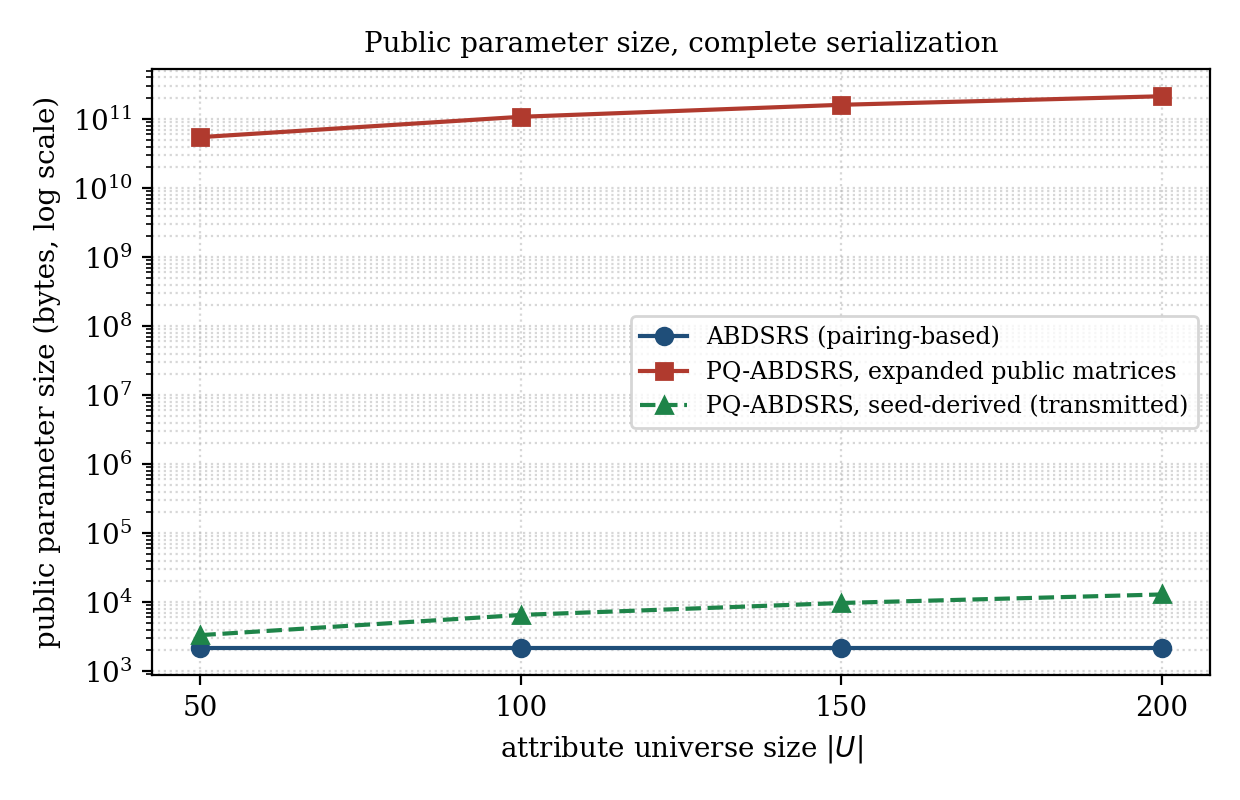
\includegraphics[width=0.85\linewidth]{Figures/size-params.png}
\caption{Public parameter size against attribute universe size, on a logarithmic axis. The
expanded curve is the working-memory and arithmetic cost; the seeded curve is what is
transmitted when the public matrices are derived from a seed
(Remark~\ref{rem:seeds}). Neither figure substitutes for the other.}
\label{fig:size-params}
\end{figure}

\begin{figure}[htbp]
\centering
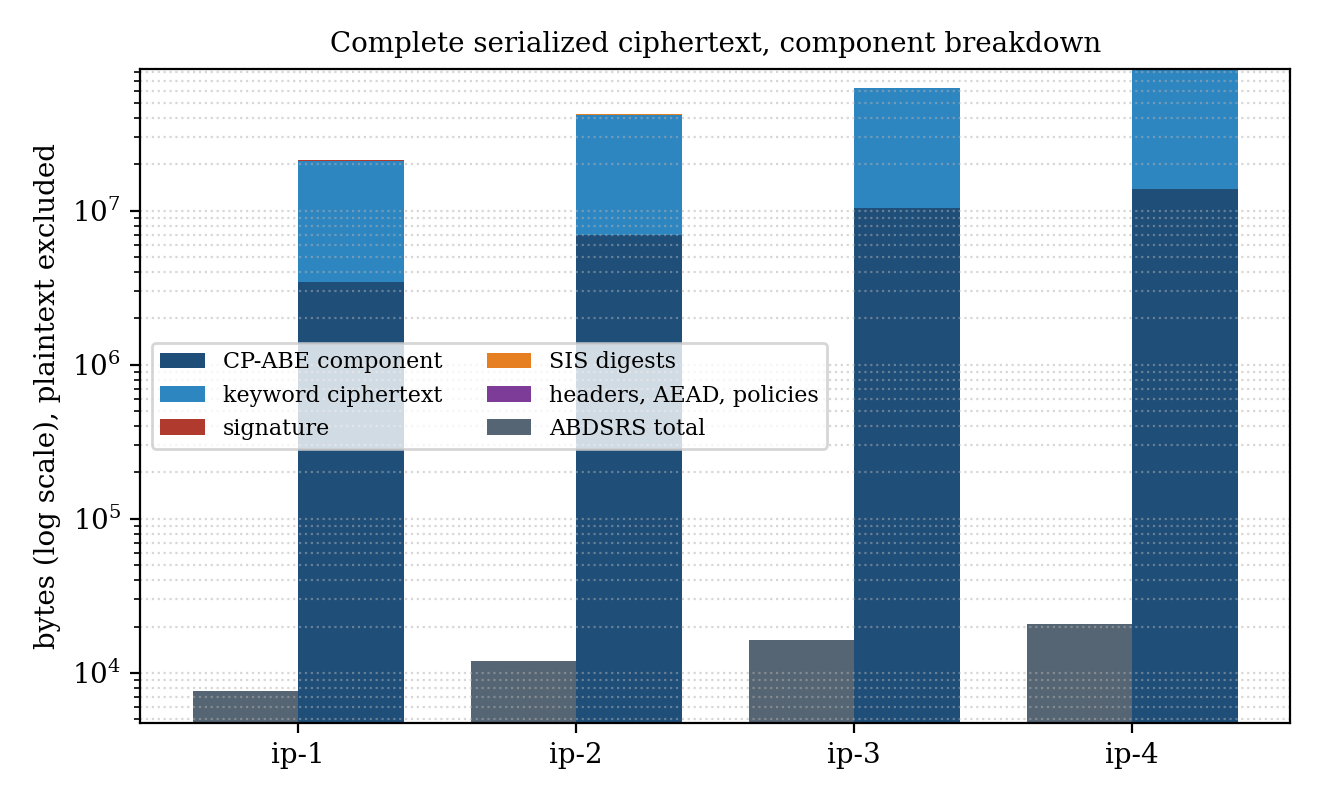
\includegraphics[width=0.9\linewidth]{Figures/size-ciphertext.png}
\caption{Complete serialized ciphertext of PQ-ABDSRS by component, against the ABDSRS total,
on a logarithmic axis. Every component listed in Algorithm~\ref{alg:onsigncrypt} is included. The PQ-ABDSRS
ciphertext is between $2{,}829$ and $4{,}031$ times larger than ABDSRS's across the four
parameter points, and the keyword layer is the dominant component throughout.}
\label{fig:size-ciphertext}
\end{figure}

\subsection{Discussion of the size gap}

The figures above are substantially worse than those reported in earlier versions of this
work, for seven reasons that we set out plainly. The dimension was corrected upward from
$n=512$ to $n=1536$, because the smaller set provides roughly $2^{41}$ rather than $2^{164}$
classical core-SVP security. The matrix width was corrected from $m\approx6{,}900$ to
$m = 2nh$, since the former did not satisfy the stated bound. The modulus was raised from
$2^{27}$ to $2^{30}$, because the correctness condition~\eqref{eq:noise} was never evaluated
in the earlier version and does not hold at $2^{27}$ for these dimensions. Key vectors were
corrected from width $m$ to width $2m$, which is the width of the matrix they invert. The decryption key became a matrix in $\Z^{2m\times\kappa}$ rather than a vector in
$\Z^{2m}$, because encapsulating $\kappa$ payload bits against a single target leaks all but
one of them (Remark~\ref{rem:dimmodel}). The keyword ciphertext was corrected to scale with
$|U^{\circ}|$ rather than with the number of keywords, which is how encryption to an attribute
vector works in the LWE key-policy ABE we instantiate (Section~\ref{subsec:kpabe}); this alone
multiplies the ciphertext by roughly four. Most importantly, the ciphertext figures of the
earliest version counted only a few scalars and one commitment, omitting the clause
ciphertexts, the keyword ciphertext, the signature and the policy descriptions. Once every
component is counted, the PQ-ABDSRS ciphertext is several thousand times larger than
ABDSRS's, not smaller. The earlier claim that PQ ciphertexts are smaller than ABDSRS's was an
artifact of those omissions and is withdrawn.

\subsection{Limitations}
\label{subsec:limits}

The public parameters are the decisive obstacle. At $|U|=100$ they occupy more than $100$ GB
expanded, which no realistic deployment will hold in working memory, and the seeded
representation of Remark~\ref{rem:seeds} reduces transmission but not computation. This is the well-known cost of unstructured LWE, and it is the reason the practical
lattice-cryptography literature works over structured lattices. The keyword layer is the
second obstacle: because the LWE key-policy ABE encrypts to an attribute vector over the whole
keyword-name universe, $\mathsf{ct}_W$ alone accounts for more than $80\%$ of the ciphertext
at every parameter point, and it does not shrink when few keywords are set.

Beyond size, four limitations follow from Section~\ref{subsec:scope}: the policy class is
restricted to DNF, with a blow-up for formulas whose DNF form is large; confidentiality is
IND-CPA rather than IND-CCA2; all proofs are in the classical random oracle model; and
negative search results are not verifiable (Remark~\ref{rem:verifscope}). The $\DRR$ also
reveals to the cloud which DNF clause the requesting user satisfies, which is stated in
Section~\ref{subsec:keywords} rather than treated as no leakage.

\subsection{Structured-lattice variant as future work}
\label{subsec:structured}

Replacing $\Zq^{n\times m}$ matrices by elements of a cyclotomic ring
$R_q := \Zq[x]/(x^{N}+1)$, or by rank-$d$ modules over such a ring, is the standard route to
smaller public parameters~\cite{lyubashevsky2010ideal,langlois2015module}. A ring element
occupies $N\lceil\log_2 q\rceil$ bits rather than $nm\lceil\log_2 q\rceil$, so the reduction
in public-parameter size would be several orders of magnitude.

We do not present such a variant as an instantiated scheme, and it appears in no comparison
table in this paper. Three things would have to be established first. The building blocks of
Section~\ref{sec:blocks} would have to be replaced by structured-lattice CP-ABE, KP-ABE and
ABS constructions with proofs under Ring-LWE or Module-LWE; reference~\cite{lyubashevsky2010ideal}
introduces Ring-LWE but supplies no attribute-based construction, and we do not attribute one
to it. The correctness bound of Theorem~\ref{thm:correctness} would have to be re-derived over
$R_q$, where the relevant norm is the expansion factor of ring multiplication rather than the
Euclidean norm of a vector. Finally, the concrete hardness would have to be re-estimated,
since the parameter set of Section~\ref{subsec:params} is not a ring parameter set and the
term ``Kyber-scale'' used in the earlier version does not describe it. We identify this as
the priority for subsequent work, together with a reference implementation to replace the
analytic figures above with measured benchmarks.

%=================================================================
\section{Conclusion}
\label{sec:conclusion}

We presented PQ-ABDSRS, an attribute-based verifiable data storage and retrieval scheme built
entirely on lattice assumptions, as a post-quantum counterpart to
ABDSRS~\cite{bera2023designing}. Access control is obtained from a lattice CP-ABE for
monotone DNF policies, keyword-policy search from a lattice KP-ABE, and data-owner
authentication and anonymity from a lattice attribute-based signature, each used through the
interface specified in Section~\ref{sec:blocks}. For non-interactive verifiability we showed
that an additively homomorphic SIS commitment does not authenticate an outsourced
computation, and we replaced it with a SIS-based binding digest bound into the data owner's
signature, together with a random-oracle preimage check on the search predicate. We isolated the decryption-error condition the composition requires, used it to fix the
modulus, and proved IND-CPA confidentiality, EUF-CMA unforgeability, verifiability, signer
privacy and keyword indistinguishability in the classical random oracle model, recording
separately in Table~\ref{tab:inherited} which guarantees are inherited from cited building
blocks.

The concrete cost is the main finding. At a parameter set giving $2^{164}$ classical and
$2^{149}$ quantum core-SVP security, the public parameters exceed ABDSRS's by more than seven orders of magnitude and the
complete ciphertext by a factor of roughly $2{,}800$ to $4{,}000$. Unstructured
LWE therefore
does not yield a deployable scheme at this functionality level, and the value of the
construction is that it establishes what a faithful migration requires and where the cost
falls, rather than that it is ready to use. Priorities for further work are a
structured-lattice re-instantiation with re-derived proofs
(Section~\ref{subsec:structured}), a chosen-ciphertext variant via a Fujisaki--Okamoto
transform (Remark~\ref{rem:cca}), a treatment in the quantum random oracle model, verifiable
handling of negative search results (Remark~\ref{rem:verifscope}), attribute revocation, and
a reference implementation.

\vspace{6pt}
%=================================================================
% "software" below refers to the analytic reproduction code accompanying this paper,
% not to an implementation of the scheme. Remove it if that code is not published.
\authorcontributions{Conceptualization, K.S. and S.K.; methodology, K.S. and S.K.; software, K.S.; formal analysis, K.S., S.K. and M.A.; investigation, K.S., S.K., M.A. and A.R.W.S.; writing---original draft preparation, K.S., S.K. and M.A.; writing---review and editing, K.S., S.K., M.A. and A.R.W.S.; visualization, K.S. and S.K.; supervision, K.S. and S.K.; project administration, M.A.; funding acquisition, M.A. and A.R.W.S. All authors have read and agreed to the published version of the manuscript.}

% ACTION REQUIRED BEFORE SUBMISSION: replace <GRANT NUMBER> with the approved grant number
% from King Faisal University, or, if the work was not externally funded, replace the whole
% \funding{...} argument with: This research received no external funding.
\funding{This work was supported by the Deanship of Scientific Research, Vice Presidency for Graduate Studies and Scientific Research, King Faisal University, Saudi Arabia, under Grant No. \hl{<GRANT NUMBER>}.}

% If the reproduction repository is NOT published, replace the text below with:
%   Data sharing is not applicable to this article as no new data were created or
%   analyzed in this study.
\dataavailability{No new data were created or analyzed in this study. The code that regenerates every parameter, table and figure reported in this article, together with the test suite that checks the reported numbers against them, is openly available at \url{https://github.com/keshavsinha/pq-abdsrs} (accessed on 16 September 2026).}

\conflictsofinterest{The authors declare no conflicts of interest.}

\reftitle{References}

%=================================================================
\begin{thebibliography}{999}
\sloppy

\bibitem{bera2023designing}
Bera, S.; Prasad, S.; Rao, Y.S.; Das, A.K.; Park, Y. Designing attribute-based verifiable data storage and retrieval scheme in cloud computing environment. \textit{J. Inf. Secur. Appl.} \textbf{2023}, \textit{75}, 103482. https://doi.org/10.1016/j.jisa.2023.103482.

\bibitem{bethencourt2007ciphertext}
Bethencourt, J.; Sahai, A.; Waters, B. Ciphertext-policy attribute-based encryption. In Proceedings of the 2007 IEEE Symposium on Security and Privacy (SP'07), Berkeley, CA, USA, 20--23 May 2007; pp. 321--334.

\bibitem{waters2011ciphertext}
Waters, B. Ciphertext-policy attribute-based encryption: An expressive, efficient, and provably secure realization. In Proceedings of Public Key Cryptography (PKC 2011), Taormina, Italy, 6--9 March 2011; Lecture Notes in Computer Science 6571; Springer: Berlin/Heidelberg, Germany, 2011; pp. 53--70.

\bibitem{zheng2014vabks}
Zheng, Q.; Xu, S.; Ateniese, G. VABKS: Verifiable attribute-based keyword search over outsourced encrypted data. In Proceedings of IEEE INFOCOM 2014, Toronto, ON, Canada, 27 April--2 May 2014; pp. 522--530.

\bibitem{sun2016protecting}
Sun, W.; Yu, S.; Lou, W.; Hou, Y.T.; Li, H. Protecting your right: Verifiable attribute-based keyword search with fine-grained owner-enforced search authorization in the cloud. \textit{IEEE Trans. Parallel Distrib. Syst.} \textbf{2016}, \textit{27}, 1187--1198.

\bibitem{cui2018efficient}
Cui, H.; Wan, Z.; Deng, R.H.; Wang, G.; Li, Y. Efficient and expressive keyword search over encrypted data in cloud. \textit{IEEE Trans. Dependable Secur. Comput.} \textbf{2018}, \textit{15}, 409--422.

\bibitem{miao2021privacy}
Miao, Y.; Liu, X.; Choo, K.K.R.; Deng, R.H.; Li, J.; Li, H.; Ma, J. Privacy-preserving attribute-based keyword search in shared multi-owner setting. \textit{IEEE Trans. Dependable Secur. Comput.} \textbf{2021}, \textit{18}, 1080--1094.

\bibitem{miao2021multi}
Miao, Y.; Deng, R.H.; Liu, X.; Choo, K.K.R.; Wu, H.; Li, H. Multi-authority attribute-based keyword search over encrypted cloud data. \textit{IEEE Trans. Dependable Secur. Comput.} \textbf{2021}, \textit{18}, 1667--1680.

\bibitem{ali2022verifiable}
Ali, M.; Sadeghi, M.R.; Liu, X.; Miao, Y.; Vasilakos, A.V. Verifiable online/offline multi-keyword search for cloud-assisted industrial Internet of Things. \textit{J. Inf. Secur. Appl.} \textbf{2022}, \textit{65}, 103101.

\bibitem{rao2016efficient}
Rao, Y.S.; Dutta, R. Efficient attribute-based signature and signcryption realizing expressive access structures. \textit{Int. J. Inf. Secur.} \textbf{2016}, \textit{15}, 81--109.

\bibitem{rao2017attribute}
Rao, Y.S. Attribute-based online/offline signcryption scheme. \textit{Int. J. Commun. Syst.} \textbf{2017}, \textit{30}, e3322.

\bibitem{deng2018ciphertext}
Deng, F.; Wang, Y.; Peng, L.; Xiong, H.; Geng, J.; Qin, Z. Ciphertext-policy attribute-based signcryption with verifiable outsourced designcryption for sharing personal health records. \textit{IEEE Access} \textbf{2018}, \textit{6}, 39473--39486.

\bibitem{belguith2020proud}
Belguith, S.; Kaaniche, N.; Hammoudeh, M.; Dargahi, T. PROUD: Verifiable privacy-preserving outsourced attribute-based signcryption supporting access policy update for cloud-assisted IoT applications. \textit{Future Gener. Comput. Syst.} \textbf{2020}, \textit{111}, 899--918.

\bibitem{maji2011attribute}
Maji, H.K.; Prabhakaran, M.; Rosulek, M. Attribute-based signatures. In Proceedings of Topics in Cryptology (CT-RSA 2011), San Francisco, CA, USA, 14--18 February 2011; Lecture Notes in Computer Science 6558; Springer: Berlin/Heidelberg, Germany, 2011; pp. 376--392.

\bibitem{boyen2013attribute}
Boyen, X. Attribute-based functional encryption on lattices. In Proceedings of the Theory of Cryptography Conference (TCC 2013), Tokyo, Japan, 3--6 March 2013; Lecture Notes in Computer Science 7785; Springer: Berlin/Heidelberg, Germany, 2013; pp. 122--142.

\bibitem{gvw2013attribute}
Gorbunov, S.; Vaikuntanathan, V.; Wee, H. Attribute-based encryption for circuits. In Proceedings of the Forty-Fifth Annual ACM Symposium on Theory of Computing (STOC 2013), Palo Alto, CA, USA, 1--4 June 2013; pp. 545--554.

\bibitem{bggh2014fkhe}
Boneh, D.; Gentry, C.; Gorbunov, S.; Halevi, S.; Nikolaenko, V.; Segev, G.; Vaikuntanathan, V.; Vinayagamurthy, D. Fully key-homomorphic encryption, arithmetic circuit ABE and compact garbled circuits. In Proceedings of EUROCRYPT 2014, Copenhagen, Denmark, 11--15 May 2014; Lecture Notes in Computer Science 8441; Springer: Berlin/Heidelberg, Germany, 2014; pp. 533--556.

\bibitem{abb2010efficient}
Agrawal, S.; Boneh, D.; Boyen, X. Efficient lattice (H)IBE in the standard model. In Proceedings of EUROCRYPT 2010, French Riviera, France, 30 May--3 June 2010; Lecture Notes in Computer Science 6110; Springer: Berlin/Heidelberg, Germany, 2010; pp. 553--572.

\bibitem{zhang2012ciphertext}
Zhang, J.; Zhang, Z.; Ge, A. Ciphertext policy attribute-based encryption from lattices. In Proceedings of the 7th ACM Symposium on Information, Computer and Communications Security (ASIACCS 2012), Seoul, Republic of Korea, 2--4 May 2012; pp. 16--17. Note: this construction supports AND-gate access policies with wildcards; it does not support arbitrary monotone span programs.

\bibitem{tsabary2019fully}
Tsabary, R. Fully secure attribute-based encryption for $t$-CNF from LWE. In Proceedings of CRYPTO 2019, Santa Barbara, CA, USA, 18--22 August 2019; Lecture Notes in Computer Science 11692; Springer: Cham, Switzerland, 2019; pp. 62--85. Note: the supported access structure is $t$-CNF, not arbitrary monotone span programs.

\bibitem{gentry2008trapdoors}
Gentry, C.; Peikert, C.; Vaikuntanathan, V. Trapdoors for hard lattices and new cryptographic constructions. In Proceedings of the Fortieth Annual ACM Symposium on Theory of Computing (STOC 2008), Victoria, BC, Canada, 17--20 May 2008; pp. 197--206.

\bibitem{chkp2010bonsai}
Cash, D.; Hofheinz, D.; Kiltz, E.; Peikert, C. Bonsai trees, or how to delegate a lattice basis. \textit{J. Cryptol.} \textbf{2012}, \textit{25}, 601--639.

\bibitem{alwen2011generating}
Alwen, J.; Peikert, C. Generating shorter bases for hard random lattices. \textit{Theory Comput. Syst.} \textbf{2011}, \textit{48}, 535--553.

\bibitem{mp2012trapdoors}
Micciancio, D.; Peikert, C. Trapdoors for lattices: Simpler, tighter, faster, smaller. In Proceedings of EUROCRYPT 2012, Cambridge, UK, 15--19 April 2012; Lecture Notes in Computer Science 7237; Springer: Berlin/Heidelberg, Germany, 2012; pp. 700--718.

\bibitem{boyen2010lattice}
Boyen, X. Lattice mixing and vanishing trapdoors: A framework for fully secure short signatures and more. In Proceedings of Public Key Cryptography (PKC 2010), Paris, France, 26--28 May 2010; Lecture Notes in Computer Science 6056; Springer: Berlin/Heidelberg, Germany, 2010; pp. 499--517.

\bibitem{tsabary2017abs}
Tsabary, R. An equivalence between attribute-based signatures and homomorphic signatures, and new constructions for both. In Proceedings of the Theory of Cryptography Conference (TCC 2017), Baltimore, MD, USA, 12--15 November 2017; Lecture Notes in Computer Science 10678; Springer: Cham, Switzerland, 2017; pp. 489--518.

\bibitem{ek2018abs}
El Kaafarani, A.; Katsumata, S. Attribute-based signatures for unbounded circuits in the ROM and efficient instantiations from lattices. In Proceedings of Public Key Cryptography (PKC 2018), Rio de Janeiro, Brazil, 25--29 March 2018; Lecture Notes in Computer Science 10770; Springer: Cham, Switzerland, 2018; pp. 89--119.

\bibitem{regev2009lattices}
Regev, O. On lattices, learning with errors, random linear codes, and cryptography. \textit{J. ACM} \textbf{2009}, \textit{56}, 1--40. Note: the worst-case to average-case reduction cited here is quantum.

\bibitem{peikert2009publickey}
Peikert, C. Public-key cryptosystems from the worst-case shortest vector problem. In Proceedings of the Forty-First Annual ACM Symposium on Theory of Computing (STOC 2009), Bethesda, MD, USA, 31 May--2 June 2009; pp. 333--342.

\bibitem{ajtai1996generating}
Ajtai, M. Generating hard instances of lattice problems. In Proceedings of the Twenty-Eighth Annual ACM Symposium on Theory of Computing (STOC 1996), Philadelphia, PA, USA, 22--24 May 1996; pp. 99--108.

\bibitem{kawachi2008commitment}
Kawachi, A.; Tanaka, K.; Xagawa, K. Concurrently secure identification schemes based on the worst-case hardness of lattice problems. In Proceedings of ASIACRYPT 2008, Melbourne, Australia, 7--11 December 2008; Lecture Notes in Computer Science 5350; Springer: Berlin/Heidelberg, Germany, 2008; pp. 372--389.

\bibitem{baum2018commitments}
Baum, C.; Damg{\aa}rd, I.; Lyubashevsky, V.; Oechsner, S.; Peikert, C. More efficient commitments from structured lattice assumptions. In Proceedings of Security and Cryptography for Networks (SCN 2018), Amalfi, Italy, 5--7 September 2018; Lecture Notes in Computer Science 11035; Springer: Cham, Switzerland, 2018; pp. 368--385.

\bibitem{gennaro2013fhma}
Gennaro, R.; Wichs, D. Fully homomorphic message authenticators. In Proceedings of ASIACRYPT 2013, Bengaluru, India, 1--5 December 2013; Lecture Notes in Computer Science 8270; Springer: Berlin/Heidelberg, Germany, 2013; pp. 301--320. Note: this work constructs a symmetric-key homomorphic authenticator, not a commitment scheme.

\bibitem{gorbunov2015leveled}
Gorbunov, S.; Vaikuntanathan, V.; Wichs, D. Leveled fully homomorphic signatures from standard lattices. In Proceedings of the Forty-Seventh Annual ACM Symposium on Theory of Computing (STOC 2015), Portland, OR, USA, 14--17 June 2015; pp. 469--477.

\bibitem{boneh2011random}
Boneh, D.; Dagdelen, {\"O}.; Fischlin, M.; Lehmann, A.; Schaffner, C.; Zhandry, M. Random oracles in a quantum world. In Proceedings of ASIACRYPT 2011, Seoul, Republic of Korea, 4--8 December 2011; Lecture Notes in Computer Science 7073; Springer: Berlin/Heidelberg, Germany, 2011; pp. 41--69.

\bibitem{zhandry2012qrom}
Zhandry, M. Secure identity-based encryption in the quantum random oracle model. In Proceedings of CRYPTO 2012, Santa Barbara, CA, USA, 19--23 August 2012; Lecture Notes in Computer Science 7417; Springer: Berlin/Heidelberg, Germany, 2012; pp. 758--775.

\bibitem{hhk2017fo}
Hofheinz, D.; H{\"o}velmanns, K.; Kiltz, E. A modular analysis of the Fujisaki--Okamoto transformation. In Proceedings of the Theory of Cryptography Conference (TCC 2017), Baltimore, MD, USA, 12--15 November 2017; Lecture Notes in Computer Science 10677; Springer: Cham, Switzerland, 2017; pp. 341--371.

\bibitem{cramer2003design}
Cramer, R.; Shoup, V. Design and analysis of practical public-key encryption schemes secure against adaptive chosen ciphertext attack. \textit{SIAM J. Comput.} \textbf{2003}, \textit{33}, 167--226.

\bibitem{rogaway2002aead}
Rogaway, P. Authenticated encryption with associated data. In Proceedings of the 9th ACM Conference on Computer and Communications Security (CCS 2002), Washington, DC, USA, 18--22 November 2002; pp. 98--107.

\bibitem{nist80038d}
Dworkin, M. Recommendation for Block Cipher Modes of Operation: Galois/Counter Mode (GCM) and GMAC; NIST Special Publication 800-38D; National Institute of Standards and Technology: Gaithersburg, MD, USA, 2007.

\bibitem{albrecht2015concrete}
Albrecht, M.R.; Player, R.; Scott, S. On the concrete hardness of learning with errors. \textit{J. Math. Cryptol.} \textbf{2015}, \textit{9}, 169--203.

\bibitem{alkim2016newhope}
Alkim, E.; Ducas, L.; P{\"o}ppelmann, T.; Schwabe, P. Post-quantum key exchange---a new hope. In Proceedings of the 25th USENIX Security Symposium, Austin, TX, USA, 10--12 August 2016; pp. 327--343.

\bibitem{cui2017expressive}
Cui, H.; Deng, R.H.; Liu, J.K.; Li, Y. Attribute-based encryption with expressive and authorized keyword search. In Proceedings of the Australasian Conference on Information Security and Privacy (ACISP 2017), Auckland, New Zealand, 3--5 July 2017; Lecture Notes in Computer Science 10342; Springer: Cham, Switzerland, 2017; pp. 106--126.

\bibitem{yang2020lightweight}
Yang, Y.; Liu, X.; Deng, R.H.; Li, Y. Lightweight sharable and traceable secure mobile health system. \textit{IEEE Trans. Dependable Secur. Comput.} \textbf{2020}, \textit{17}, 78--91.

\bibitem{miao2021optimized}
Miao, Y.; Deng, R.H.; Choo, K.K.R.; Liu, X.; Ning, J.; Li, H. Optimized verifiable fine-grained keyword search in dynamic multi-owner settings. \textit{IEEE Trans. Dependable Secur. Comput.} \textbf{2021}, \textit{18}, 1804--1820.

\bibitem{lyubashevsky2010ideal}
Lyubashevsky, V.; Peikert, C.; Regev, O. On ideal lattices and learning with errors over rings. In Proceedings of EUROCRYPT 2010, French Riviera, France, 30 May--3 June 2010; Lecture Notes in Computer Science 6110; Springer: Berlin/Heidelberg, Germany, 2010; pp. 1--23.

\bibitem{langlois2015module}
Langlois, A.; Stehl{\'e}, D. Worst-case to average-case reductions for module lattices. \textit{Des. Codes Cryptogr.} \textbf{2015}, \textit{75}, 565--599.

\bibitem{shor1997}
Shor, P.W. Polynomial-time algorithms for prime factorization and discrete logarithms on a quantum computer. \textit{SIAM J. Comput.} \textbf{1997}, \textit{26}, 1484--1509.

\end{thebibliography}

\PublishersNote{}
\end{document}
